

\documentclass[journal]{IEEEtran}
\usepackage{graphicx}
\usepackage{amsmath}
\usepackage{amssymb}
\usepackage{amsxtra}
\usepackage{amstext}
\usepackage{latexsym}
\usepackage{dsfont}
\usepackage{float}
\usepackage{cite}
\usepackage{subcaption}
\ifCLASSINFOpdf
%\usepackage[pdftex]{graphicx}
  % declare the path(s) where your graphic files are
  % \graphicspath{{../pdf/}{../jpeg/}}
  % and their extensions so you won't have to specify these with
  % every instance of \includegraphics
  % \DeclareGraphicsExtensions{.pdf,.jpeg,.png}
\else

\fi

\hyphenation{op-tical net-works semi-conduc-tor}


\begin{document}
\title{Optimization design and performance analysis of linear polarization antenna in 2.45 GHz on-body communications}

\author{Lingfeng~Liu,~\IEEEmembership{}
        Xiaonan~Wang,~\IEEEmembership{}
        and~Peng~Zhang.~\IEEEmembership{}% <-this % stops a space
\thanks{Lingfeng liu, Xiaonan Wang and Zhang Peng are with the Signal Information Engineering school, East China Jiaotong University, China, e-mail: lingf.liu@gmail.com.}% <-this % stops a space
\thanks{This work is supported by the Natural Science Foundation of China (NSFC) under grant No. 81460275.}% <-this % stops a space
\thanks{Manuscript submitted July 4, 2017.}}


\maketitle

\begin{abstract}
In this paper, three kinds of compact linearly polarized antennas are proposed, and the effects of horizontal polarization and vertical polarization on the polarization performance of the antenna are analyzed based on the simulation. Antennas are inverted F antenna, MIFA and printed dipole. Simulated human chest model includes skin�� fat��muscle three-tier structure. The results show that the change of resonant frequency is small after loading the human body, but the radiation orientation of the antenna is more obvious due to the coupling effect of the human body, and the bandwidth, center frequency and S11 are affected by the distance between the antenna and the body surface and the relative orientation. After loading the human body, the resonant frequency of the antenna changes little, the pattern is relatively stable.
\end{abstract}

% Note that keywords are not normally used for peerreview papers.
\begin{IEEEkeywords}
IFA, MIFA, printed dipole, horizontal polarization, vertical polarization, Body Area Network(BAN).
\end{IEEEkeywords}

\IEEEpeerreviewmaketitle



\section{Introduction}
\IEEEPARstart{R}{cent} years, the use of cellular phones and other personal communication services has gradually widened, making the focus of research on the human body wearing antennas. In the WBAN communication system, the 2.4GHz frequency band is widely used in various areas of WBAN due to the small size of the antenna, high transmission rate and low power consumption, such as health care in the monitoring and prevention of health, the detection of posture and motion in fitness and entertainment. At present, most of the research is place the antenna in the shape of  phone on human's head of the assumptions for simulation and testing\cite{1,2}. But the wearing antenna is usually placed on human body's torso or limbs, the recent studies have shown that these are optimal locations for wearable antennas\cite{3}.

In the study of the antenna on body surface, the following problems usually arise: the antenna is integrated in the clothing or placed on body surface\cite{4,5}. The human body can be seen as a media of complex characteristics and must have an impact on antenna performance parameters\cite{6,7}. At the same time the distance between antenna and body surface is also one of the important factors. In order to study the impacts of these factors on antenna performance, three kinds of linear polarized antennas were selected and placed on the surface of the human body. The antenna performance was observed by changing the distance between antenna and body surface. This paper consists of four parts, the second part introduces the selection and optimization of three kinds of linear polarized antennas and the third part introduces the performance of the antennas after loading body model. The comparison of S11 and bandwidth of different distances and antenna patterns in different polarization are also processed. Finally, the performance of the linear polarization antenna in 2.45GHz body surface communication is summarized.

\section{Design and optimization of antennas in free apace}
\subsection{IFA}
IFA is a monopole of a deformation of the structure, it has a small size, simple structure, low production costs and it's also easy to match. In this paper, the IFA is fabricated on the PCB and operates in the 2.4GHz ISM band with the center frequency of 2.45GHz. The designed antenna structure model is shown in fig. \ref{fig:1a}. Dielectric layer is made of the most commonly used glass fiber epoxy resin (FR4) in PCB, with $\epsilon_{r}$=4.4\cite{8}.
\begin{figure}[!htb]
\centering
\begin{subfigure}[b]{0.35\textwidth}
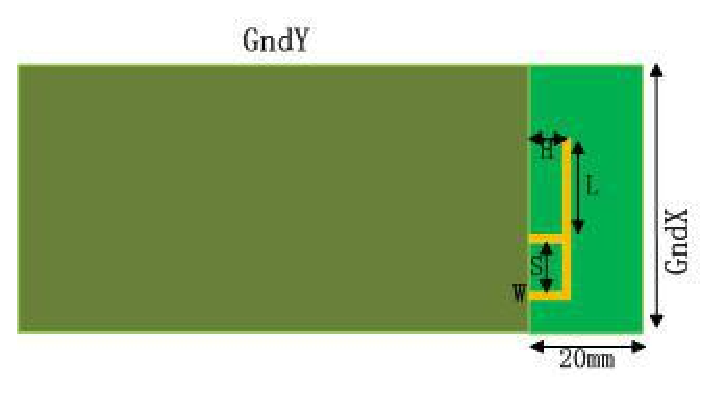
\includegraphics[width=\textwidth]{figs/1a.eps}
\caption{Parameter model }
\label{fig:1a}	
\end{subfigure}		
\begin{subfigure}[b]{0.4\textwidth}
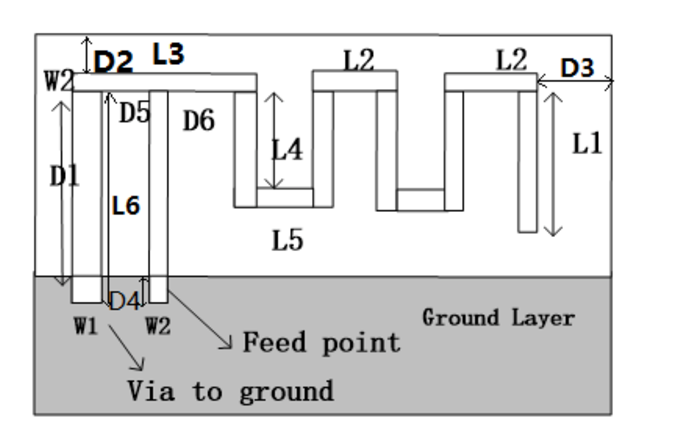
\includegraphics[width=\textwidth]{figs/1b.eps}
\caption{Optimized S11}
\label{fig:1b}
\end{subfigure}
\begin{subfigure}[b]{0.4\textwidth}
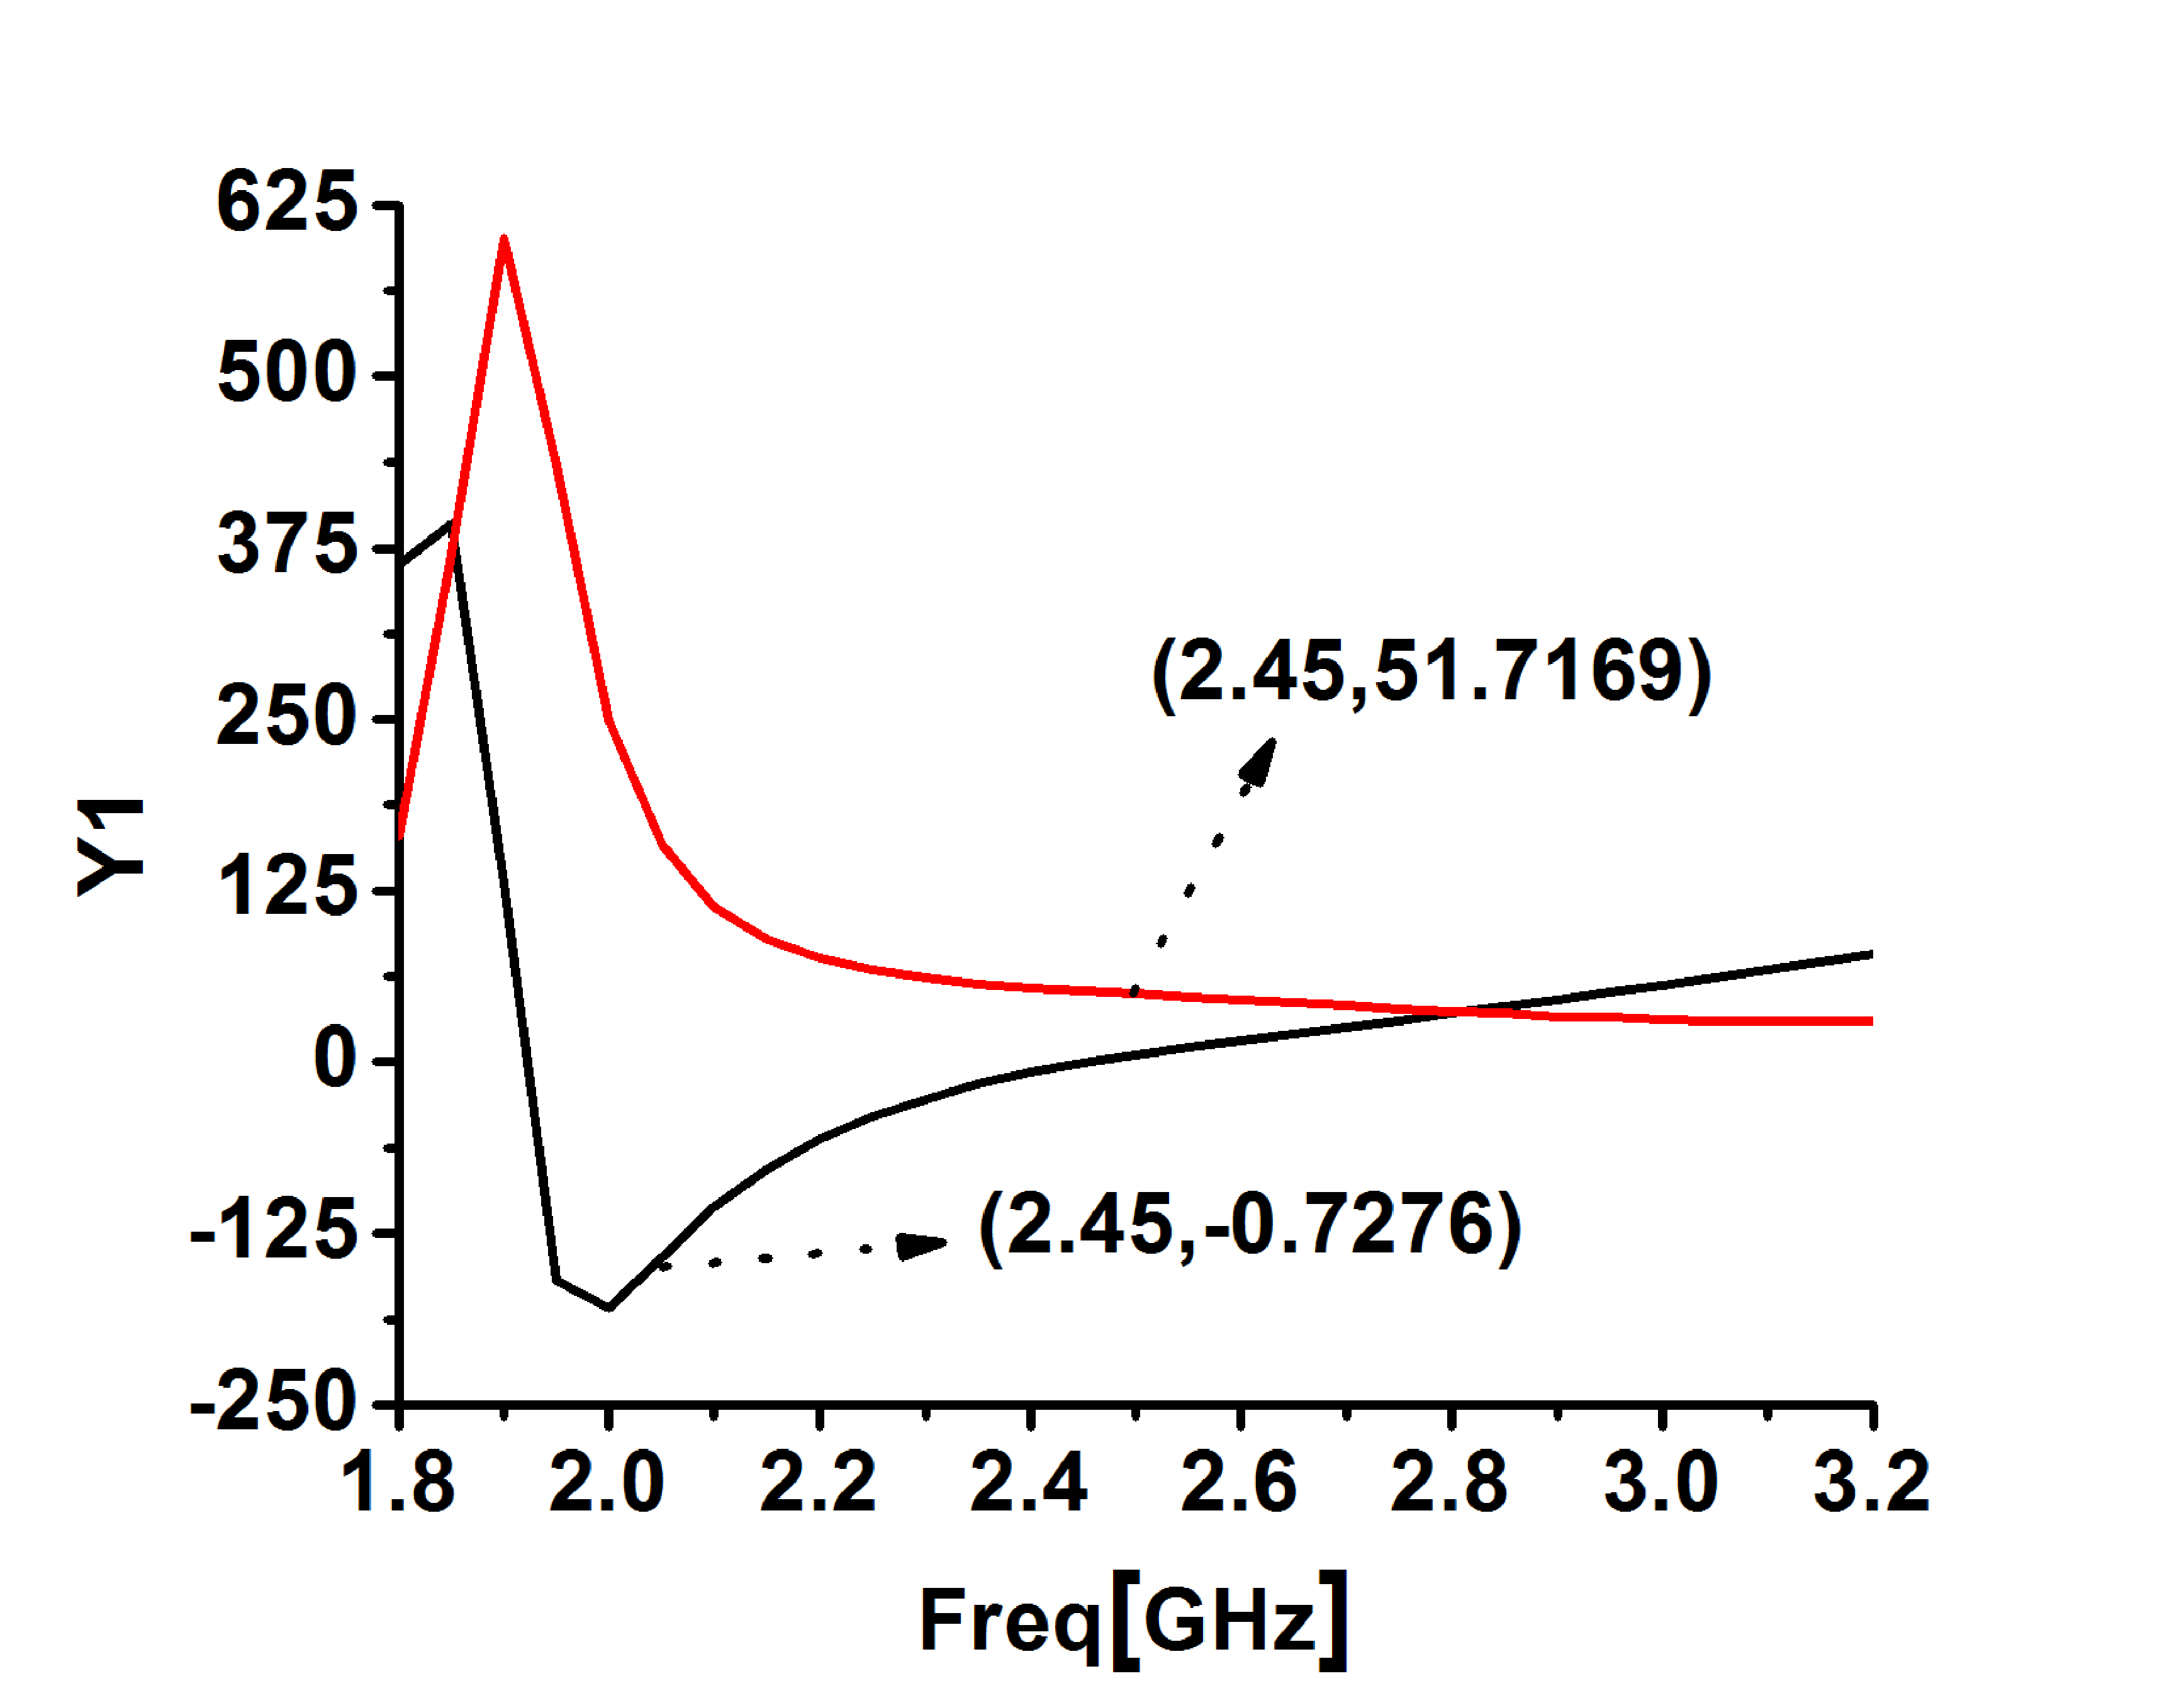
\includegraphics[width=\textwidth]{figs/1c.eps}
\caption{Optimized input impedance }
\label{fig:1c}
\end{subfigure}
\caption{Inverted-F antenna}
\label{fig:1}
\end{figure}
The antenna is simulated by Ansoft HFSS 13.0. After appropriate analysis and optimization of the values of the main parameters, when \textit{L}=16.2mm, \textit{H}=3.8mm and \textit{S}=5mm, the antenna resonant frequency is 2.45GHz, the bandwidth is about 450MHz, and the input impedance of the antenna is (50.2 + j0.35)$\Omega$ and has a good match with 50$\Omega$\cite{8}.

\subsection{MIFA}
MIFA is a common antenna and widely used in various man-machine interface devices (HID) due to its smaller PCB space and superior performance. The structure of MIFA proposed in this paper is shown in fig. \ref{fig:2a}, the dielectric layer is made of the most commonly FR4 with $\epsilon_{r}$=4.4 and a dielectric layer thickness of 0.8 mm. Its length and width were 34mm and 15.2mm, respectively. The ground point of the antenna is connected to the ground plane through a rectangular ideal conductor plane\cite{9}.

In the design process of MIFA, we use Ansoft HFSS 13.0, after the analysis and optimization of main parameters \textit{GndX} and \textit{L1}, while \textit{L1} = 3.5 and \textit{GndX} = 34 mm, the resonant frequency is around 2.45 GHz and the bandwidth is about 225 MHz.
\begin{figure}[!htb]
\centering
\begin{subfigure}[b]{0.4\textwidth}
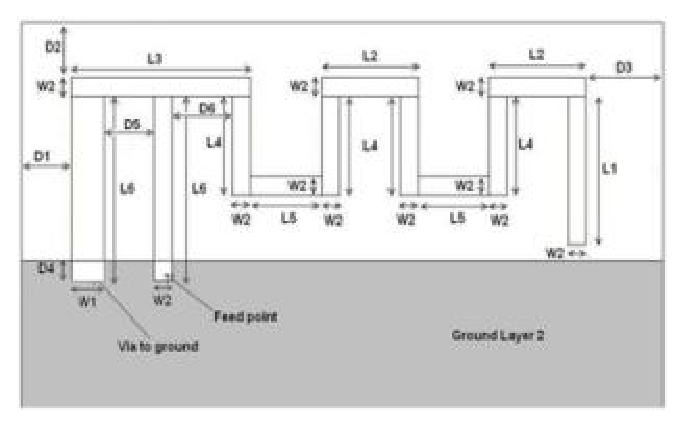
\includegraphics[width=\textwidth]{figs/2a.eps}
\caption{Parameter mode}
\label{fig:2a}	
\end{subfigure}		
\begin{subfigure}[b]{0.4\textwidth}
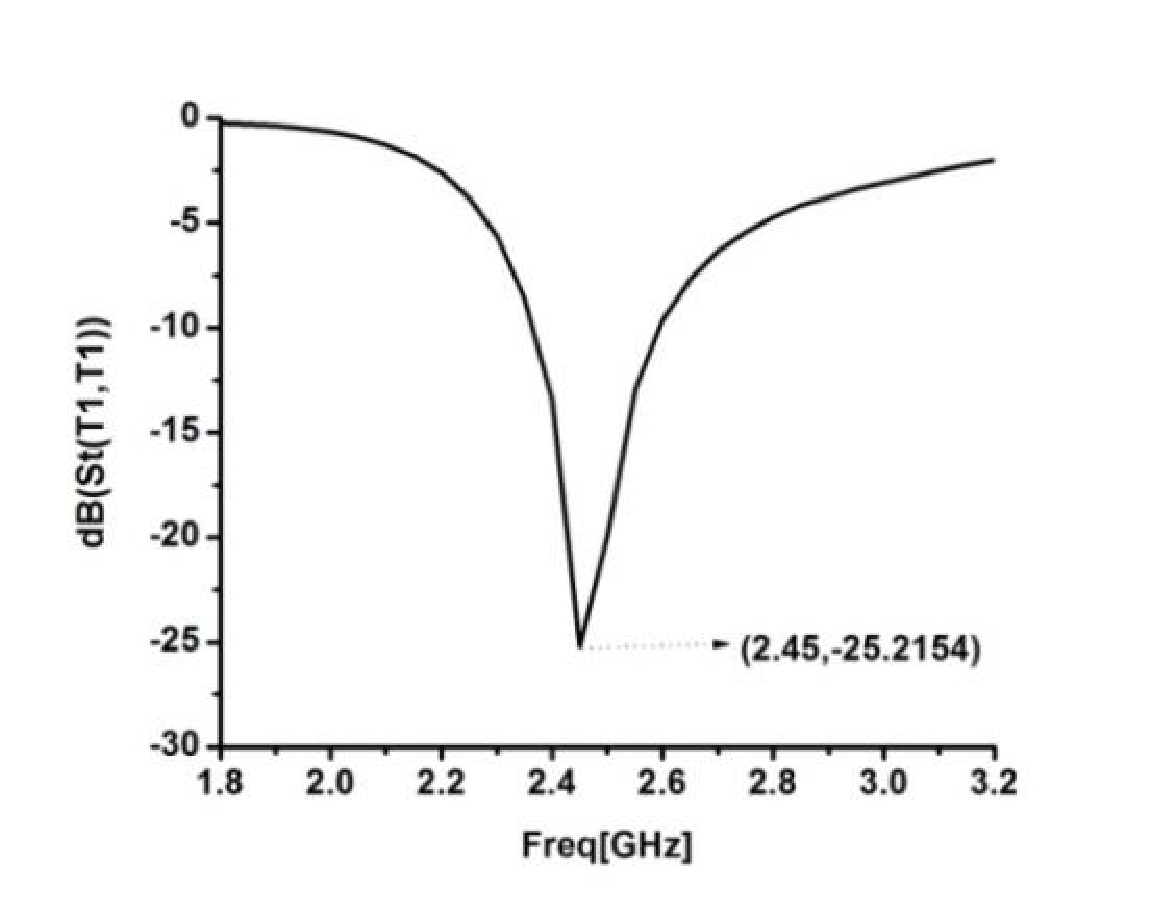
\includegraphics[width=\textwidth]{figs/2b.eps}
\caption{Optimized S11}
\label{fig:2b}
\end{subfigure}
\caption{MIFA}
\label{fig:2}
\end{figure}
\begin{figure}[!htb]
\centering
\begin{subfigure}[b]{0.35\textwidth}
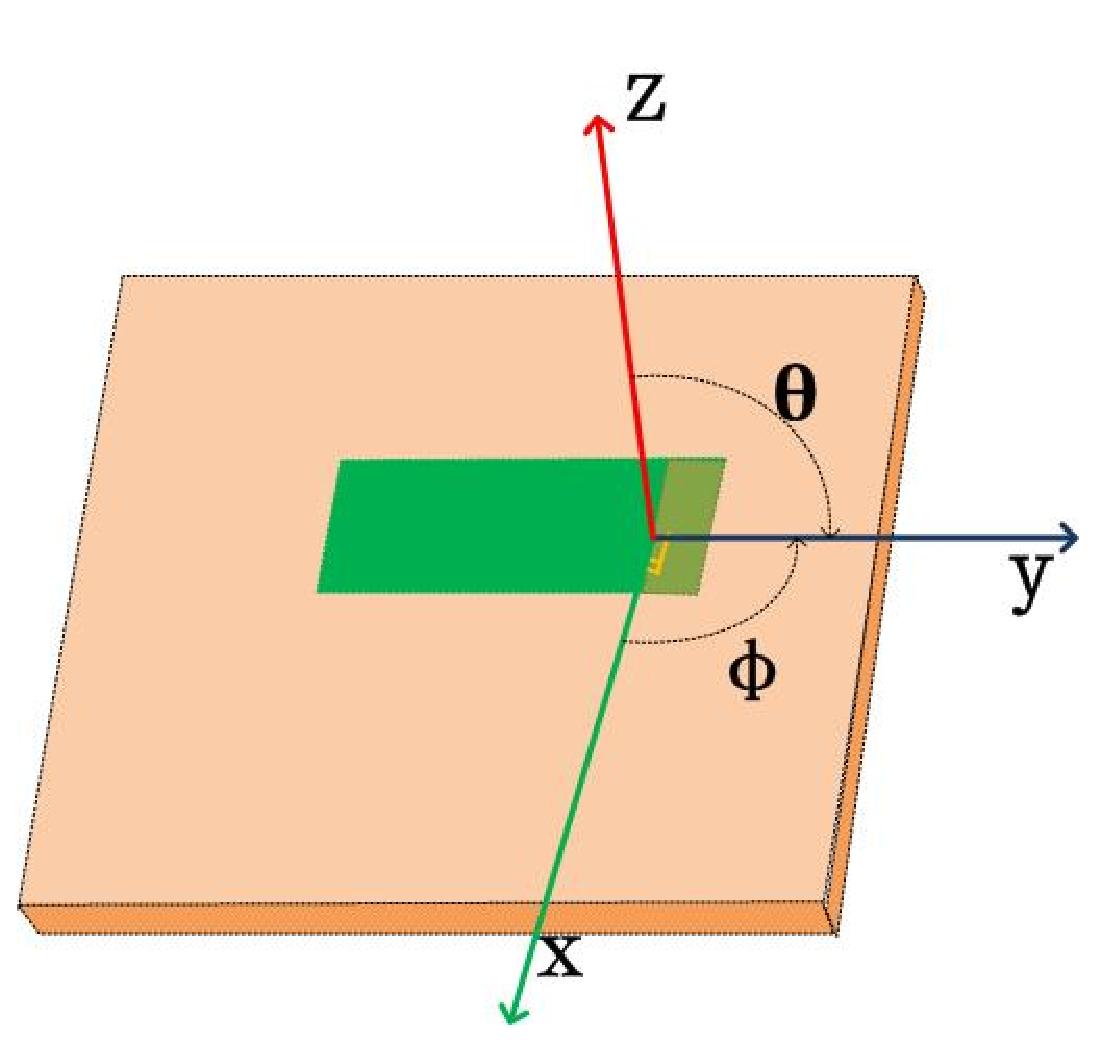
\includegraphics[width=\textwidth]{figs/3a.eps}
\caption{Parameter mode}
\label{fig:a}	
\end{subfigure}		
\begin{subfigure}[b]{0.4\textwidth}
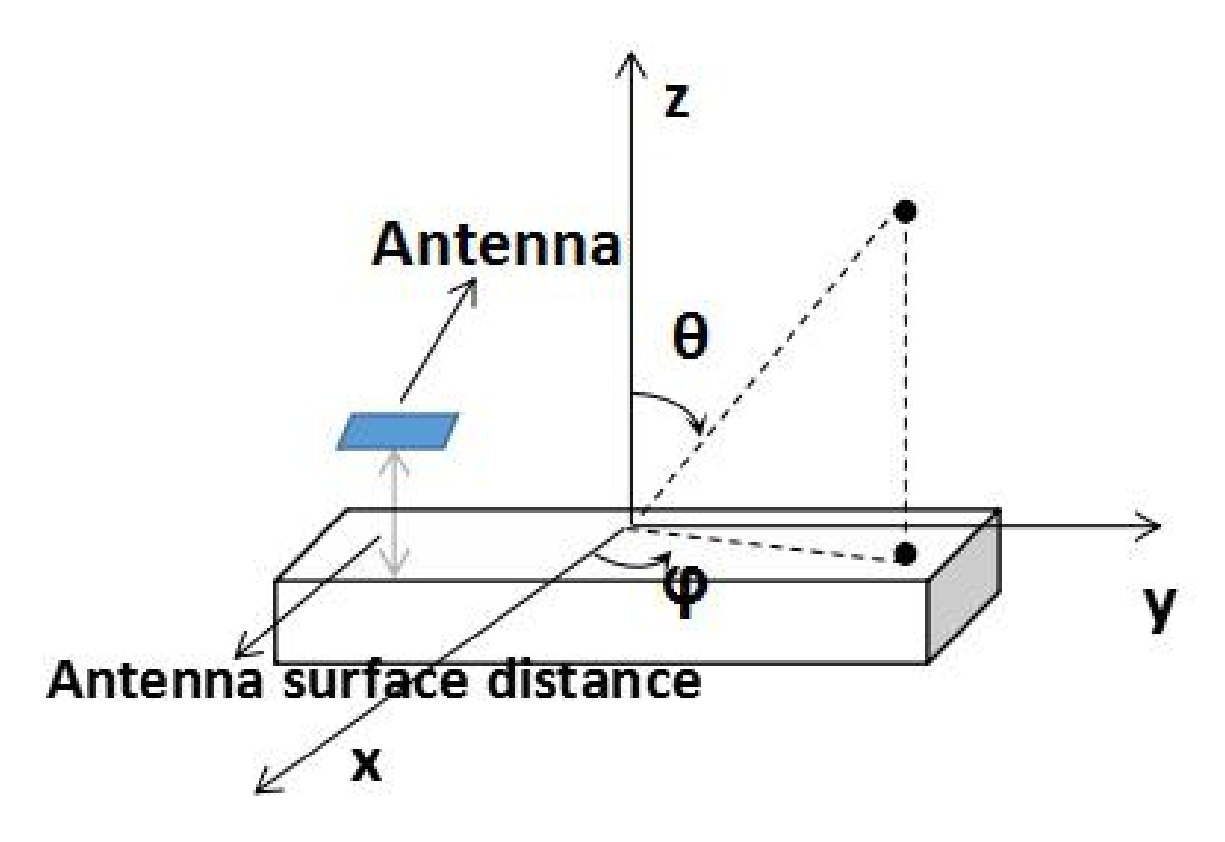
\includegraphics[width=\textwidth]{figs/3c.eps}
\caption{Optimized S11}
\label{fig:c}
\end{subfigure}
\begin{subfigure}[b]{0.4\textwidth}
\includegraphics[width=\textwidth]{figs/3b.eps}
\caption{Optimized input impedance}
\label{fig:b}	
\end{subfigure}	
\caption{MIFA}\label{fig:3}
\end{figure}

\subsection{Print Dipole}
The design of microstrip balun-fed printed dipole is a deformation of half-wave dipole antenna. The material of dielectric layer is FR4 with $\epsilon_{r}$= 4.4, and its thickness is 1.6 mm. In the design process of printed dipole, the antenna is simulated by Ansoft HFSS 13.0 and the values of the main parameters \textit{L2} and \textit{L3} are optimized and analyzed appropriately. While \textit{L2} = 21mm, \textit{L3}= 6mm, the maximum bandwidth is 550MHz and achieve a good impedance matching at 2.45GHz.

\section{Human body simulation}
We must establish the body model accurately in the study of the impact of human body on antenna, but the human body is composed of various biological tissues with different shapes and electromagnetic properties. Most of the biological tissues are non-uniform dispersion medium and human body can��t be accurately modeled. However, we can construct different human models to obtain multiple results as much as possible within allowable range of the error.

\subsection{Human body model}
In the actual measurement process of measuring antennas, it is difficult to get accurate conclusions because of the interference from external environment to antenna performance and problems from route connection, so we simulate in a state of the simulation. As the antenna is not directly in contact with body surface, we place a box simulated human chest at a certain distance from the antenna, and the box is a three layered biological tissue model\cite{10}. As shown in fig. \ref{fig:4}, the three-layer structure of the skin layer(2 mm), fat layer(5 mm) and muscle layer(10 mm) was set from top to the bottom, and the model volume was 200mm*160mm*170mm. Considering that the 2.45 GHz signal is rapidly attenuated in human body, this structure is considered to be able to adequately simulate the human body. We set dielectric constant and other electrical characteristics\cite{10} similar to human body, then analyze the polarization performance of antenna by observing simulated results.
\begin{figure}[!htb]
\centering
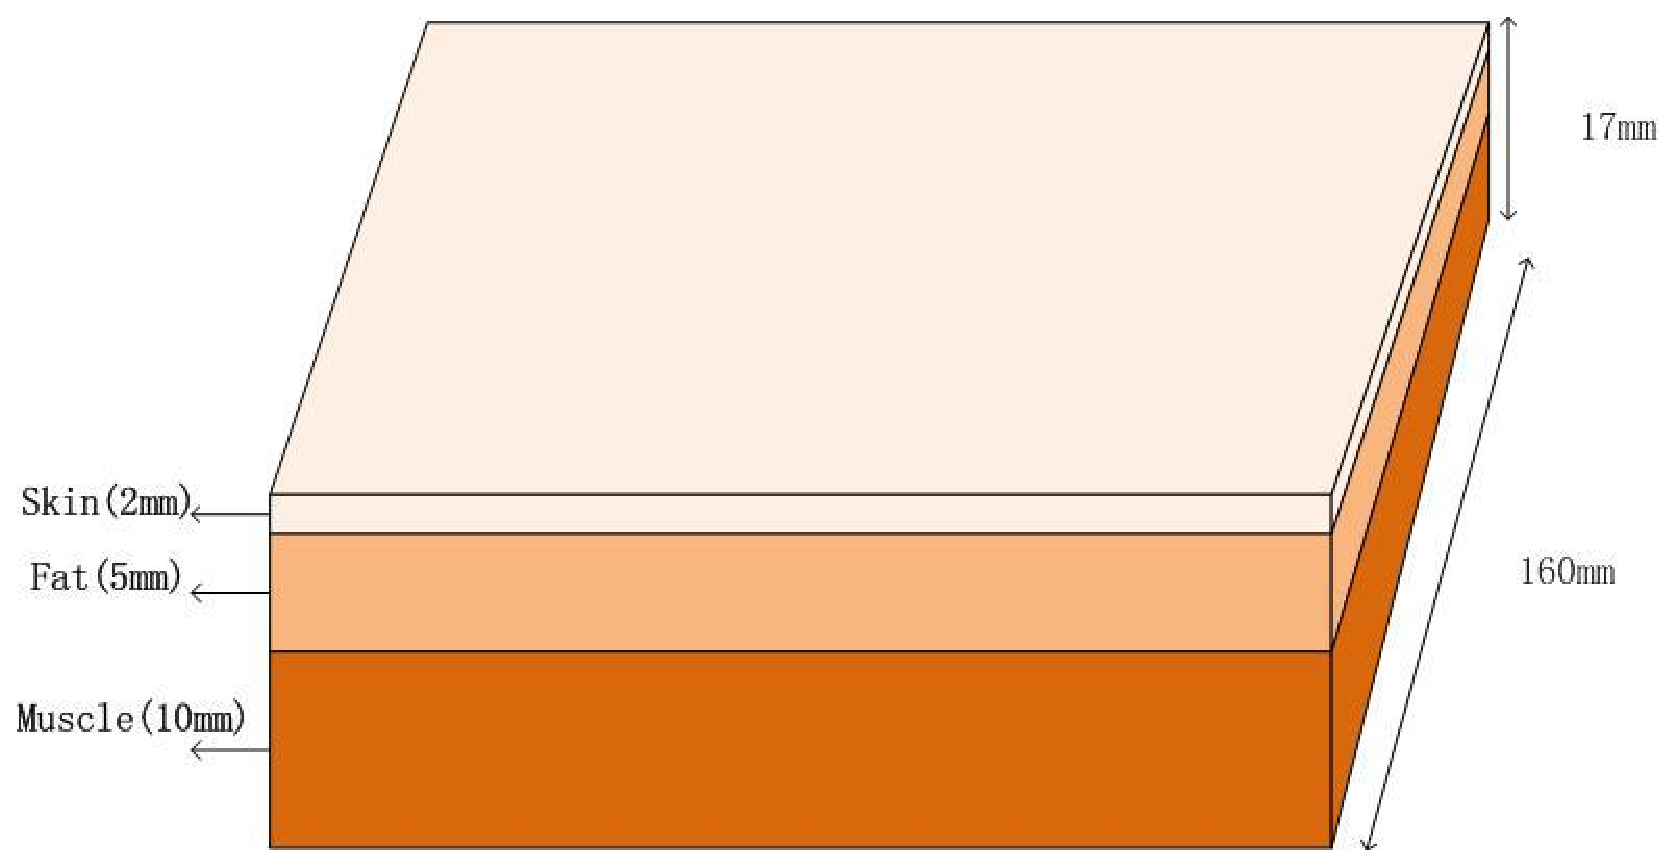
\includegraphics[width=0.4\textwidth]{figs/4.eps}
\caption{Parameter mode}
\label{fig:4}	
\end{figure}		
\begin{table}[!h]
\centering
\begin{tabular}{|c|c|c|}
\hline
Tissue&$\epsilon_{r}$&$\sigma$\\
\hline
Skin&38.0066&1.4638\\
\hline
Muscle&52.7295&1.7388\\
Fat&10.8206&0.2680\\
\hline
\end{tabular}
\caption{Electromagnetic parameters of the human body's tissues at 2.45 GHZ}
\label{tab:1}
\end{table}
% needed in second column of first page if using \IEEEpubid
%\IEEEpubidadjcol

\subsection{Comparison of antenna polarization performance}
\begin{figure}[!htb]
\centering
\begin{subfigure}[b]{0.24\textwidth}
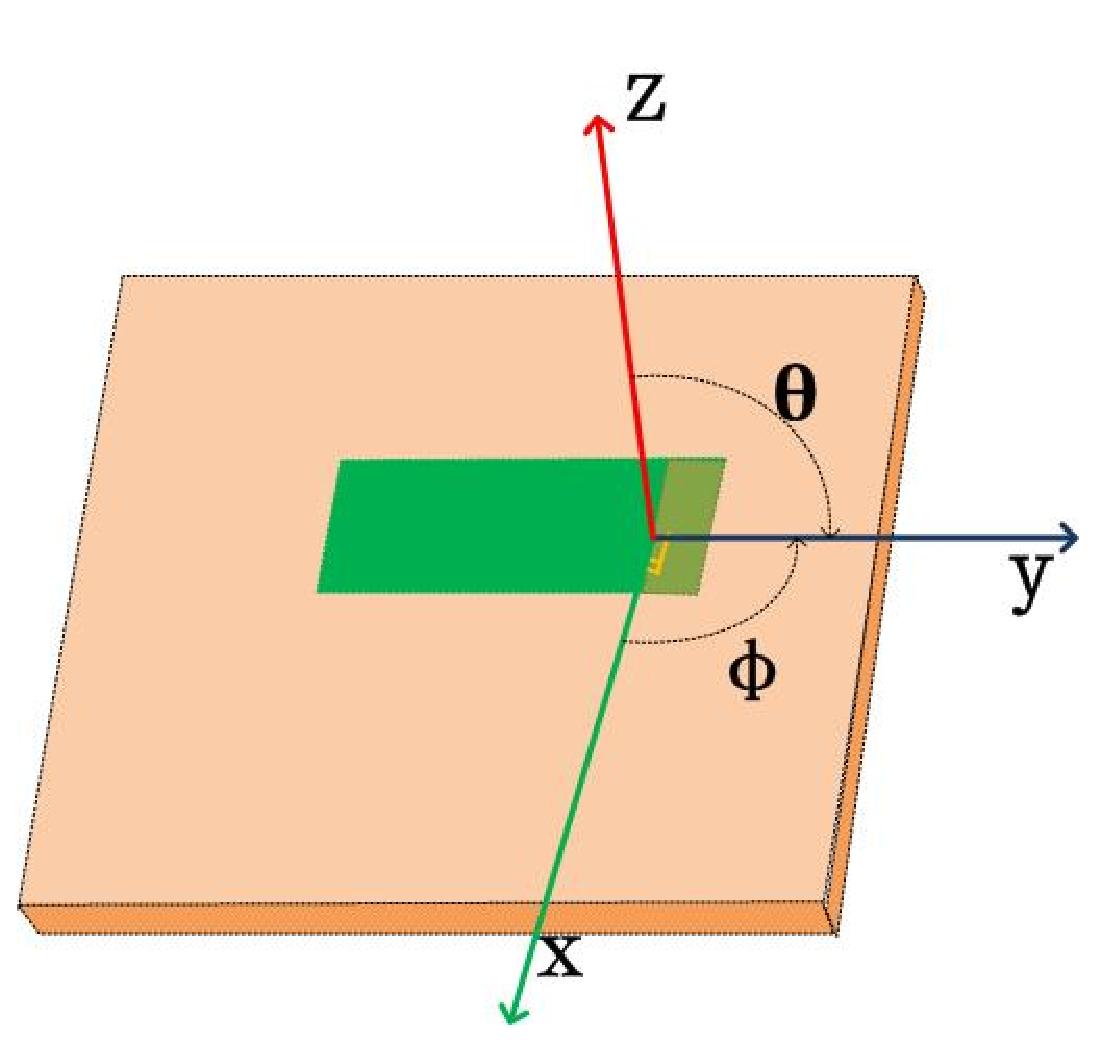
\includegraphics[width=\textwidth]{figs/5a.eps}
\caption{Horizontal polarization}
\label{fig:5a}	
\end{subfigure}		
\begin{subfigure}[b]{0.24\textwidth}
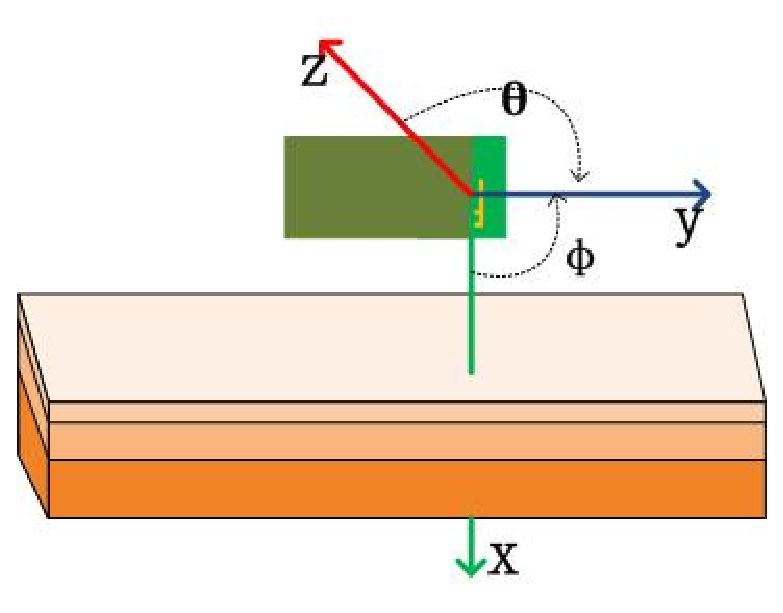
\includegraphics[width=\textwidth]{figs/5b.eps}
\caption{Vertical polarization}
\label{fig:5b}
\end{subfigure}
\caption{MIFA}
\label{fig:5}
\end{figure}
The focus of this paper is to observe the antenna performance after loading body model by changing the antenna placement. The distance between antenna and body surface is also an important factor of antenna performance. So we summarize the variation of S11 and bandwidth(B) in the range of 0.5cm$<\textit{d}<$6cm, and compare the changes of antenna gain pattern of different distances(d).

\subsubsection{IFA}
Fig. \ref{fig:6} shows the changes of antenna matching performance and bandwidth of \textit{d}. For horizontal polarization, 0.4GHz\textless\textit{B}\textless0.52GHz, when \textit{d}= 2.5cm, \textit{B} reaches the maximum; for vertical polarization, the fitting equation for the bandwidth is
\begin{equation}
\label{eq:eps_1}
y[GHz]=0.0628x+0.1845,   x[cm]
\end{equation}
\begin{figure}[!htb]
\centering
\begin{subfigure}[b]{0.4\textwidth}
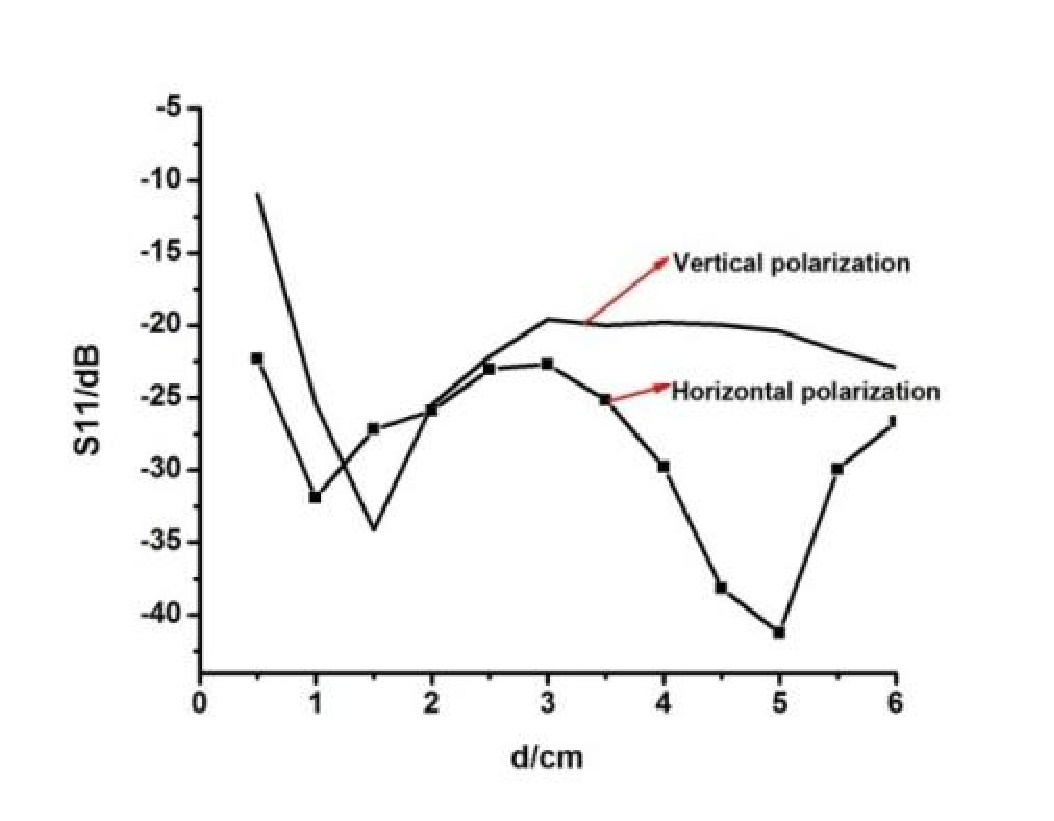
\includegraphics[width=\textwidth]{figs/6a.eps}
\caption{S11 changes}
\label{fig:a}	
\end{subfigure}		
\begin{subfigure}[b]{0.4\textwidth}
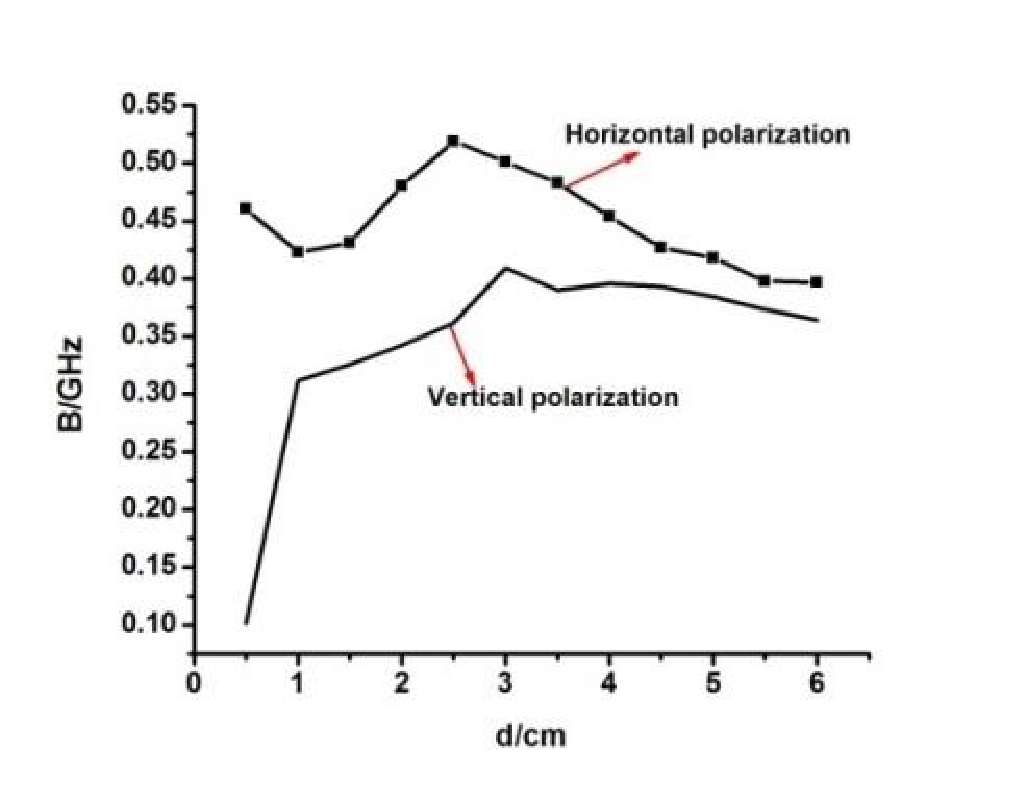
\includegraphics[width=\textwidth]{figs/6b.eps}
\caption{B changes}
\label{fig:b}
\end{subfigure}
\caption{Comparison of \textit{S11} and \textit{B} of horizontal polarization and vertical polarization with different \textit{d}}
\label{fig:6}
\end{figure}
\begin{figure}[!htb]
\centering
\begin{subfigure}[b]{0.22\textwidth}
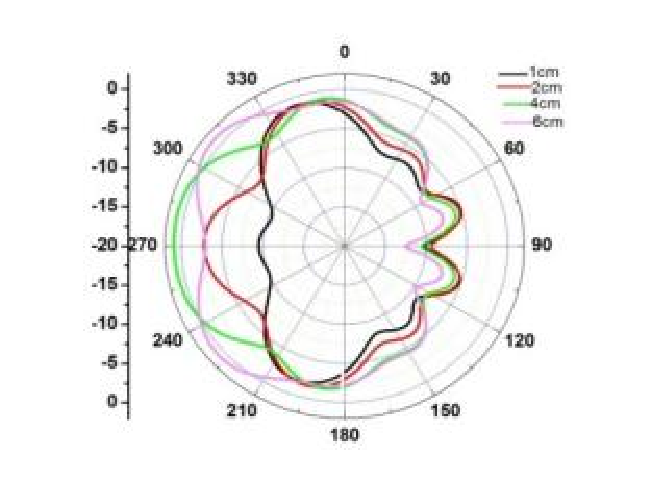
\includegraphics[width=\textwidth]{figs/7a.eps}
\caption{E(YZ) plane of horizontal polarization}
\label{fig:a}	
\end{subfigure}		
\begin{subfigure}[b]{0.22\textwidth}
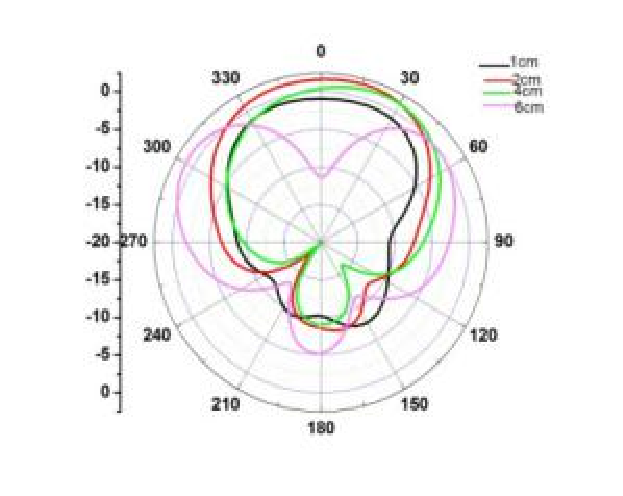
\includegraphics[width=\textwidth]{figs/7b.eps}
\caption{E plane of vertical polarization}
\label{fig:b}
\end{subfigure}
\begin{subfigure}[b]{0.22\textwidth}
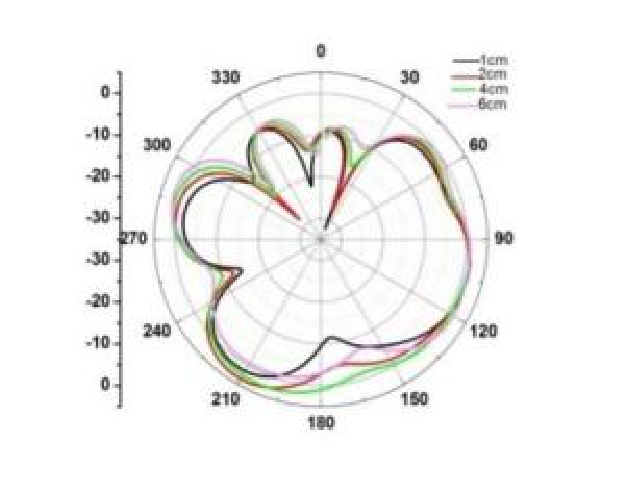
\includegraphics[width=\textwidth]{figs/7d.eps}
\caption{H(XY) plane of horizontal polarization}
\label{fig:d}	
\end{subfigure}
\begin{subfigure}[b]{0.22\textwidth}
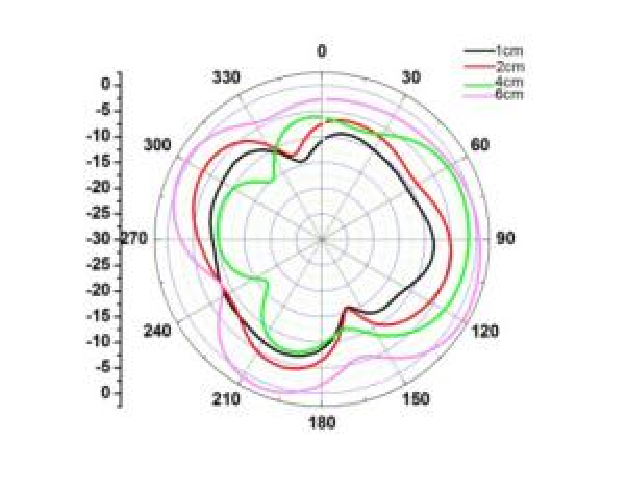
\includegraphics[width=\textwidth]{figs/7e.eps}
\caption{H plane of vertical polarization}
\label{fig:e}	
\end{subfigure}
\begin{subfigure}[b]{0.24\textwidth}
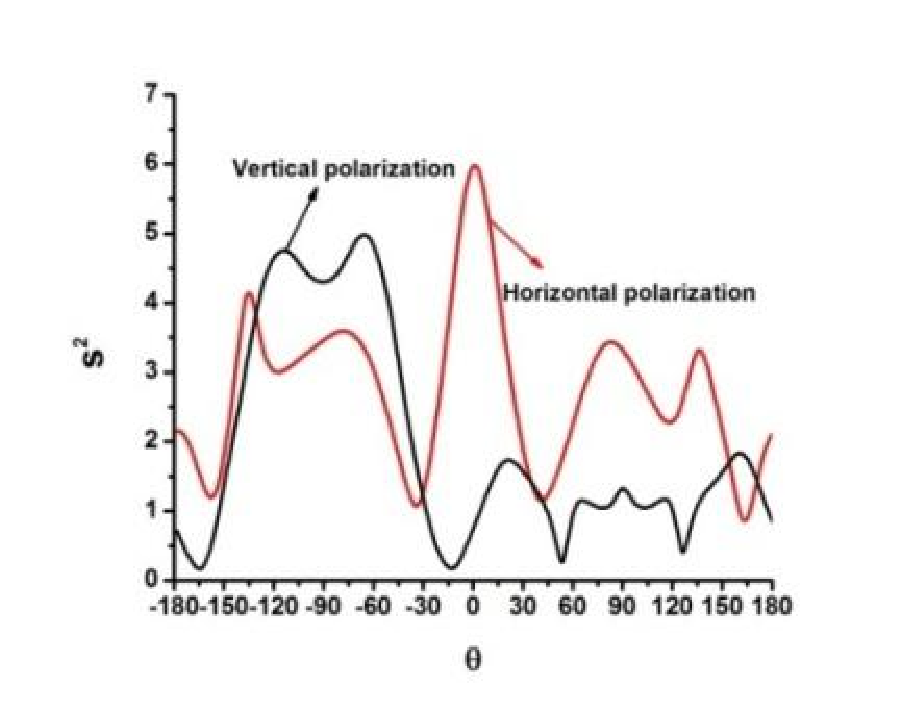
\includegraphics[width=\textwidth]{figs/7c.eps}
\caption{E-plane}
\label{fig:c}	
\end{subfigure}
\begin{subfigure}[b]{0.24\textwidth}
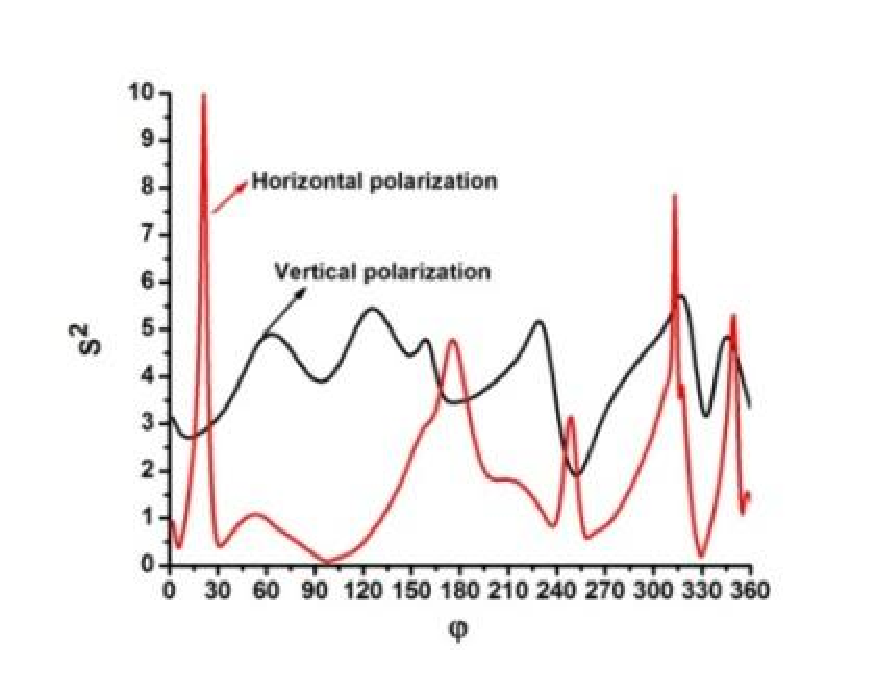
\includegraphics[width=\textwidth]{figs/7f.eps}
\caption{H-plane}
\label{fig:f}	
\end{subfigure}
\caption{Comparison of gain pattern of horizontal polarization and vertical polarization of \textit{d}}
\label{fig:7}
\end{figure}
When \textit{d}=0.5cm, the bandwidth is the narrowest, and the antenna is not suitable for placing on body surface this time. S11 of horizontal polarization decreases with the increase of d. When \textit{d}=5cm, S11 is the smallest and the antenna matching is the best; When 0.5cm\textless\textit{d}\textless1.5cm, S11 of vertical polarization decreases with the increase of \textit{d} and when \textit{d}=1.5cm, S11 reaches the minimum and the antenna matching performance is the best, when 1.5cm$<\textit{d}<$4cm, S11 increases with the increase of d, and the antenna matching performance get worse. When 0.5cm$<\textit{d}<$1.2cm, \textit{d}\textgreater2cm, the horizontal polarization of S11 is always smaller than vertical polarization and the bandwidth is always wider than vertical polarization. Therefore, horizontal polarization of the antenna performance is better than vertical polarization of this range of \textit{d}.
\begin{figure}[!htb]
\centering
\begin{subfigure}[b]{0.24\textwidth}
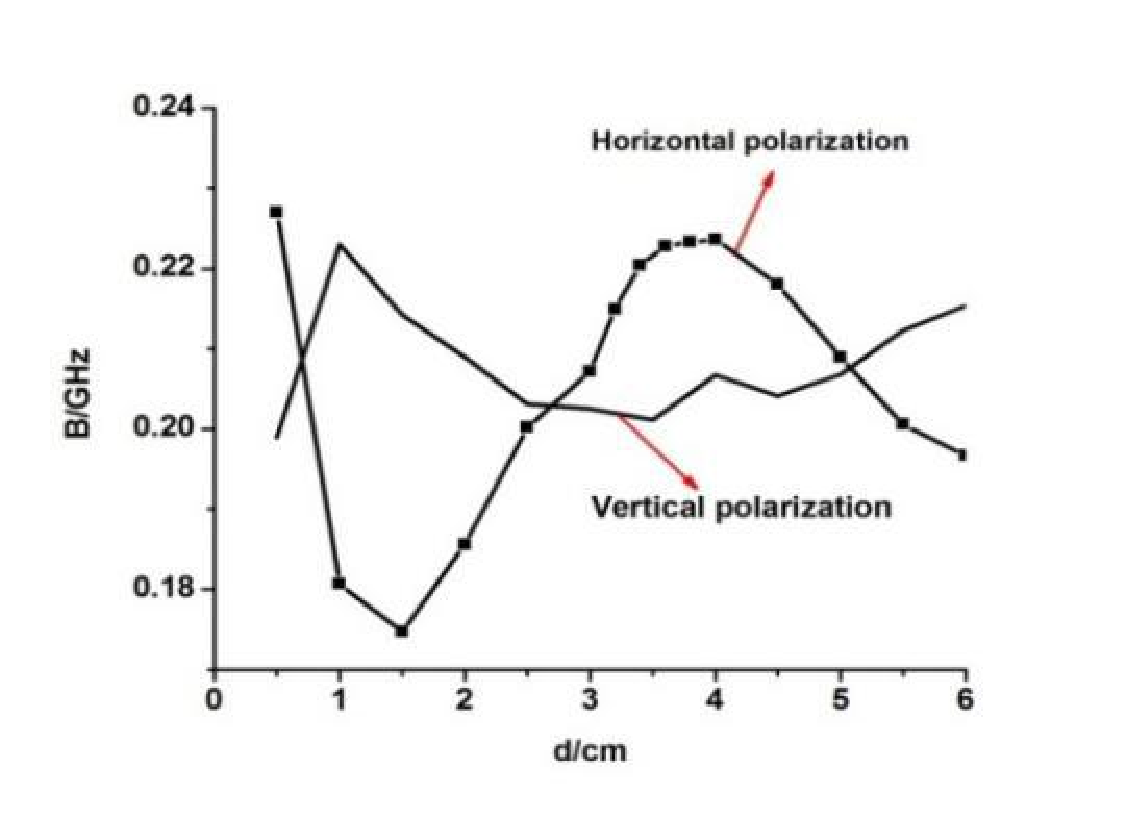
\includegraphics[width=\textwidth]{figs/8a.eps}
\caption{E-plane}
\label{fig:a}	
\end{subfigure}
\begin{subfigure}[b]{0.24\textwidth}
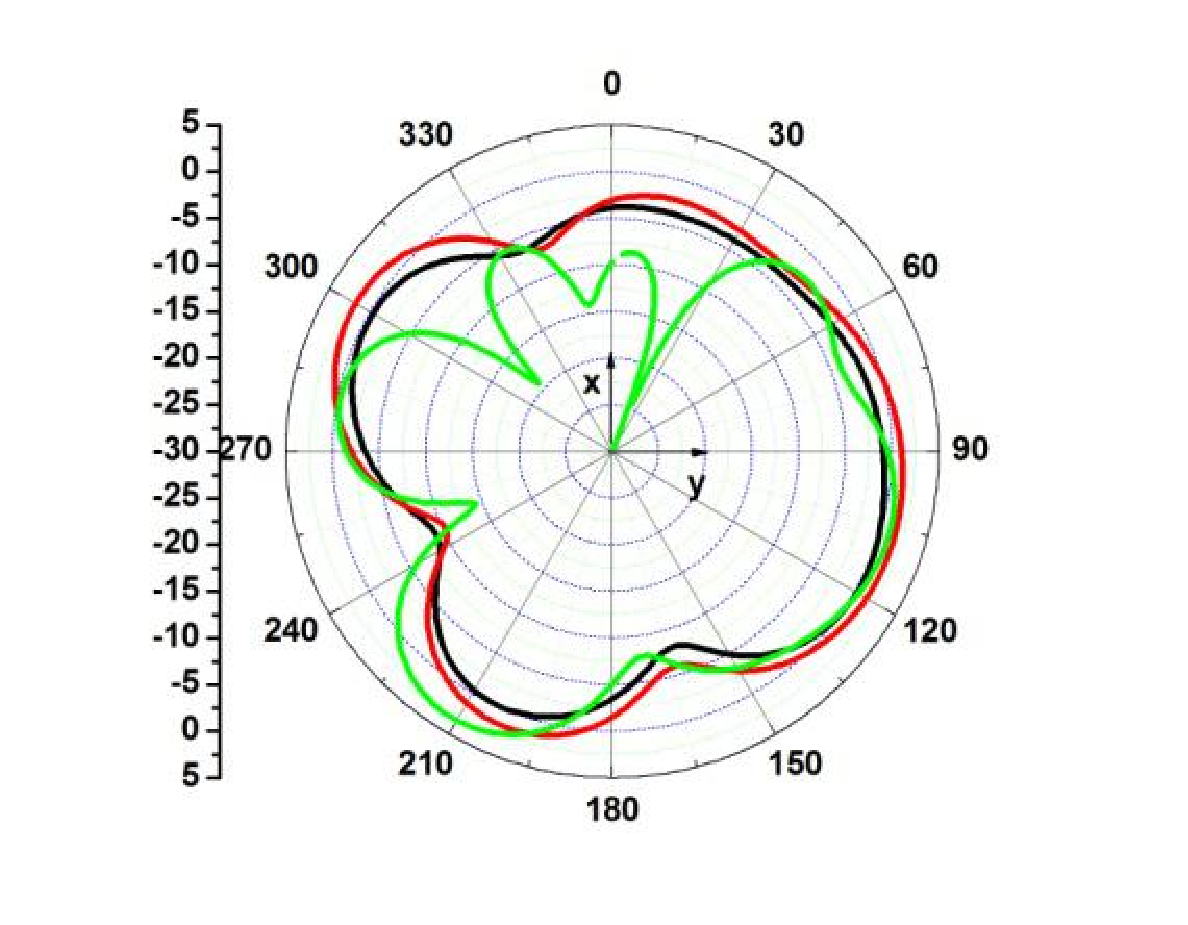
\includegraphics[width=\textwidth]{figs/8c.eps}
\caption{H-plane}
\label{fig:c}	
\end{subfigure}		
\begin{subfigure}[b]{0.23\textwidth}
\includegraphics[width=\textwidth]{figs/8b.eps}
\caption{Differential gain of E-plane }
\label{fig:b}
\end{subfigure}
\begin{subfigure}[b]{0.23\textwidth}
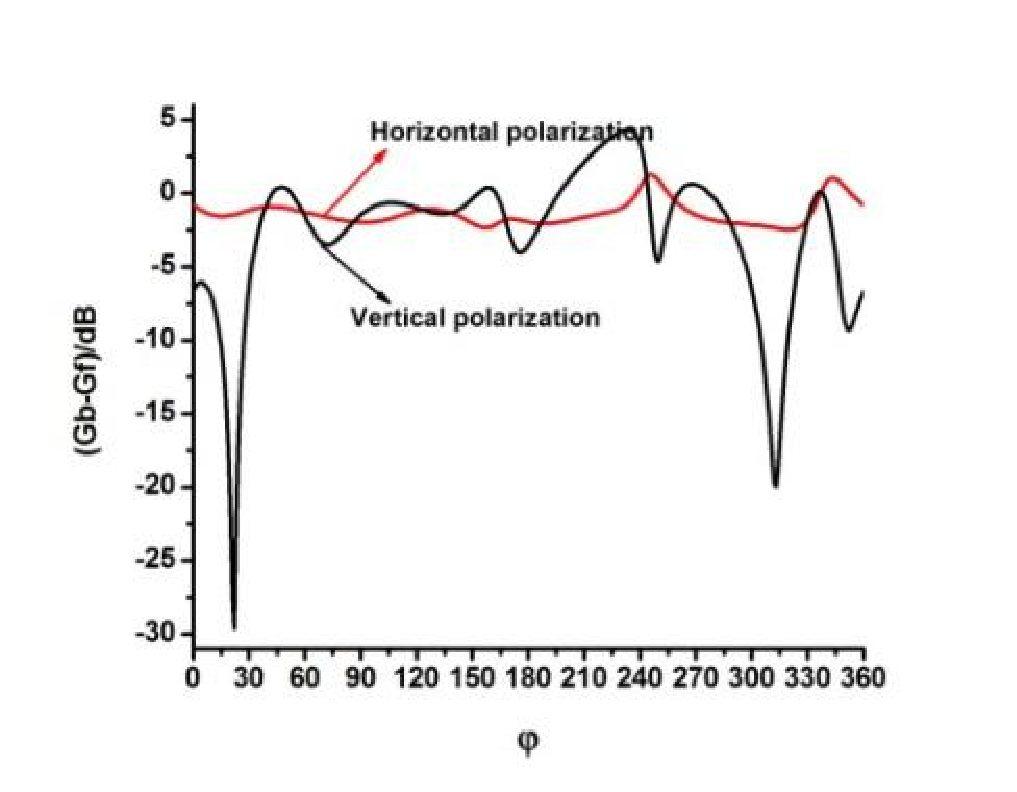
\includegraphics[width=\textwidth]{figs/8d.eps}
\caption{Differential gain of H-plane}
\label{fig:d}	
\end{subfigure}
\caption{Antenna gain pattern}
\label{fig:8}
\end{figure}

E-plane pattern of horizontal polarization is stable and not sensitive to \textit{d}. For H-plane pattern, when $0\,^{\circ}$\textless$\varphi$\textless$30\,^{\circ}$, $310\,^{\circ}$��\textless$\varphi$\textless$330\,^{\circ}$,
$S^{2}$\textgreater5, indicating that the difference between the gain in the same direction is great and antenna directional gain is sensitive to distance. The directional gain distribution of vertical polarization at different distances is relatively uniform and not sensitive to the \textit{d}.

By comparing the antenna polarization performance at different distances, it��s found that the impact on antenna is not obvious of \textit{d}. Therefore, 5cm and 1.5cm are selected as the research focus for horizontal polarization and vertical polarization, respectively.
E-plane radiation pattern of horizontal polarization and vertical polarization after loading body model are symmetrical distribution of $\theta$=$0\,^{\circ}$ and $\theta$=$90\,^{\circ}$. The fitted gain difference curve equation of horizontal polarization is
\begin{equation}
\label{eq:eps_2}
y[dB]=0.0003797+0.00488x+1.00823,  x[cm]
\end{equation}
The  body model has a great influence on the antenna gain at the position of $-180\,^{\circ}$\textless$\theta$\textless$-125\,^{\circ}$, $125\,^{\circ}$��\textless$\theta$\textless$180\,^{\circ}$, and when $\theta$=$140\,^{\circ}$, $\mid$$G_{b}$-$G_{f}$$\mid$ is the maximum and the human body has the most obvious effects on antenna. For vertical polarization, $\mid$$G_{b}$-$G_{f}$$\mid$\textless6, human body has a uniform effect on antenna gain pattern over the entire range of \textit{$\theta$}. The impact of human body to vertical polarization are more obvious than horizontal polarization.\\
H-plane pattern of horizontal polarization after loading body model is similar to omnidirectional distribution of free space. For vertical polarization, when $0\,^{\circ}$\textless$\varphi$\textless$35\,^{\circ}$, $295\,^{\circ}$\textless$\varphi$\textless$320\,^{\circ}$, $340\,^{\circ}$\textless$\varphi$\textless$360\,^{\circ}$, $\mid$$G_{b}$-$G_{f}$$\mid$\textgreater4, human body has great effects on antenna gain pattern, when $\varphi$=$17\,^{\circ}$, $\mid$$G_{b}$-$G_{f}$$\mid$ reach the maximum and human body has the most obvious effects on antenna.

\subsubsection{MIFA}
\begin{figure}[!htb]
\centering
\begin{subfigure}[b]{0.4\textwidth}
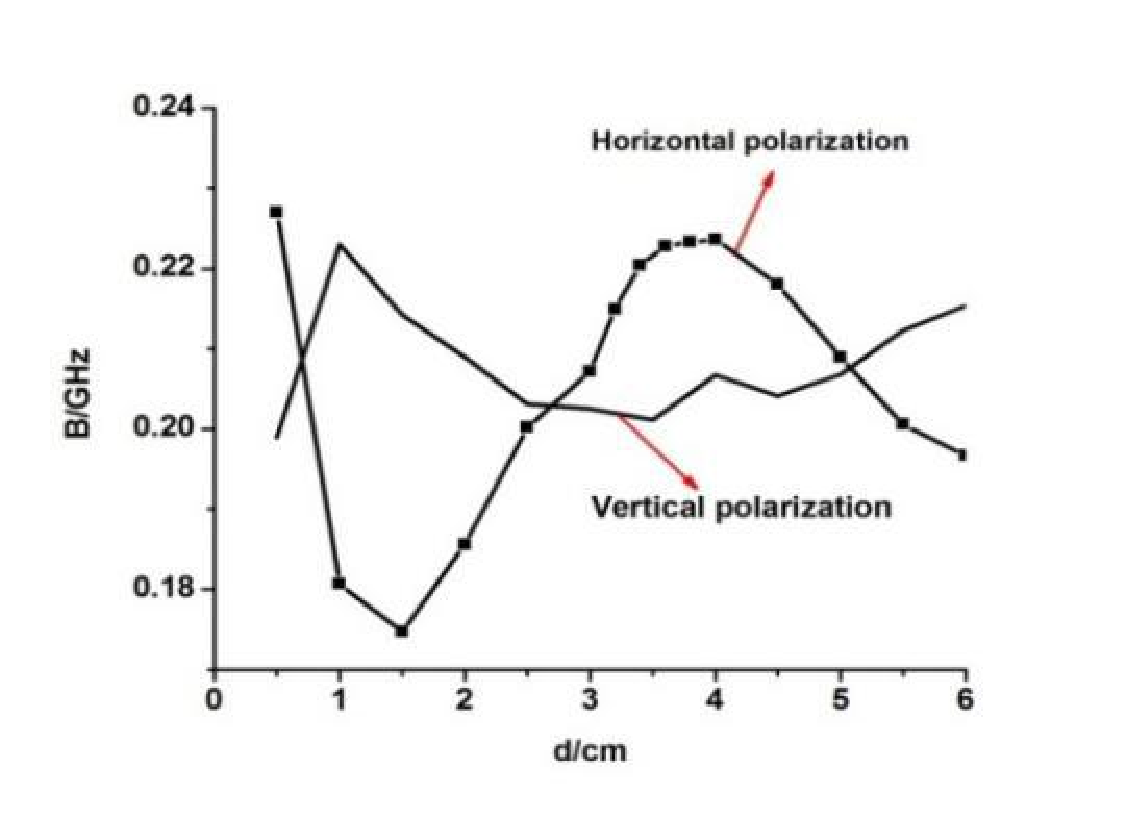
\includegraphics[width=\textwidth]{figs/9a.eps}
\caption{S11 changes}
\label{fig:a}	
\end{subfigure}		
\begin{subfigure}[b]{0.4\textwidth}
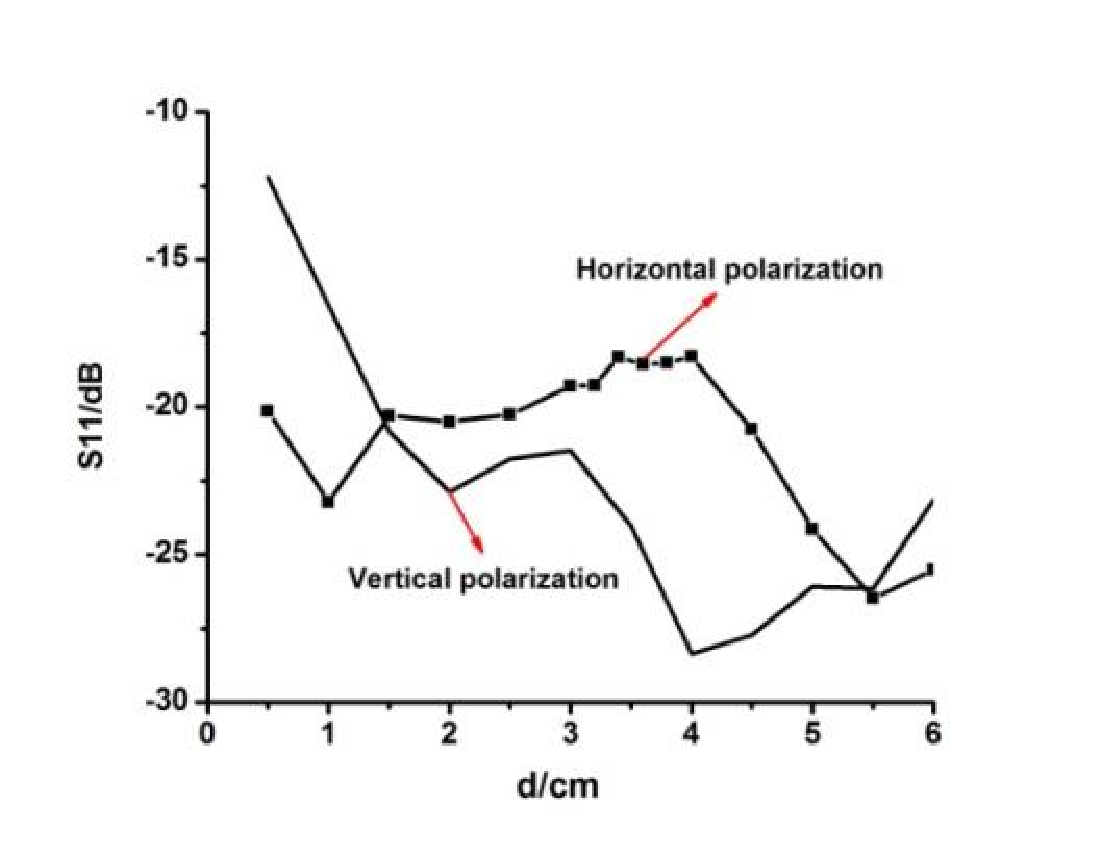
\includegraphics[width=\textwidth]{figs/9b.eps}
\caption{B changes}
\label{fig:b}
\end{subfigure}
\caption{Comparison of S11 and B of horizontal polarization and vertical polarization with different \textit{d}
}
\label{fig:9}
\end{figure}
For horizontal polarization, the fitting equation for bandwidth is
\begin{equation}
\label{eq:eps_3}
y[GHz]=-0.00178x^2+0.01416x+0.18396,  x[cm]
\end{equation}
When \textit{d}=1.5cm, the bandwidth is the narrowest, and the antenna is not suitable for placing on body surface. For horizontal polarization, the effect of distance on bandwidth is not obvious. When \textit{d}=1cm, \textit{B}=225GHz, reaching the maximum. The fitting equation for S11 of vertical polarization is
\begin{equation}
\label{eq:eps_4}
y[dB]=2.02866x-16.01,  x[cm]
\end{equation}
\begin{figure}[!htb]
\centering
\begin{subfigure}[b]{0.24\textwidth}
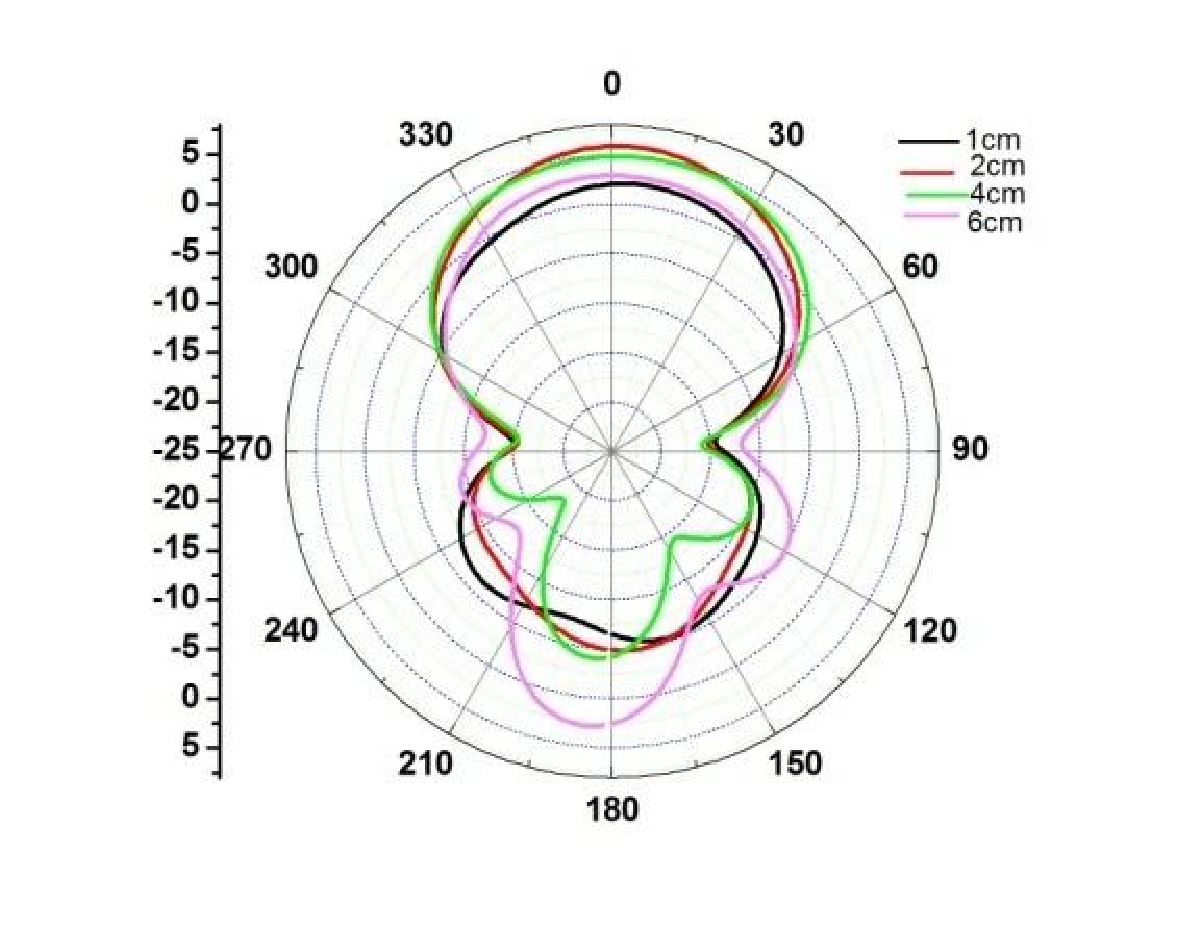
\includegraphics[width=\textwidth]{figs/10a.eps}
\caption{Horizontal polarization of E-plane}
\label{fig:a}	
\end{subfigure}		
\begin{subfigure}[b]{0.24\textwidth}
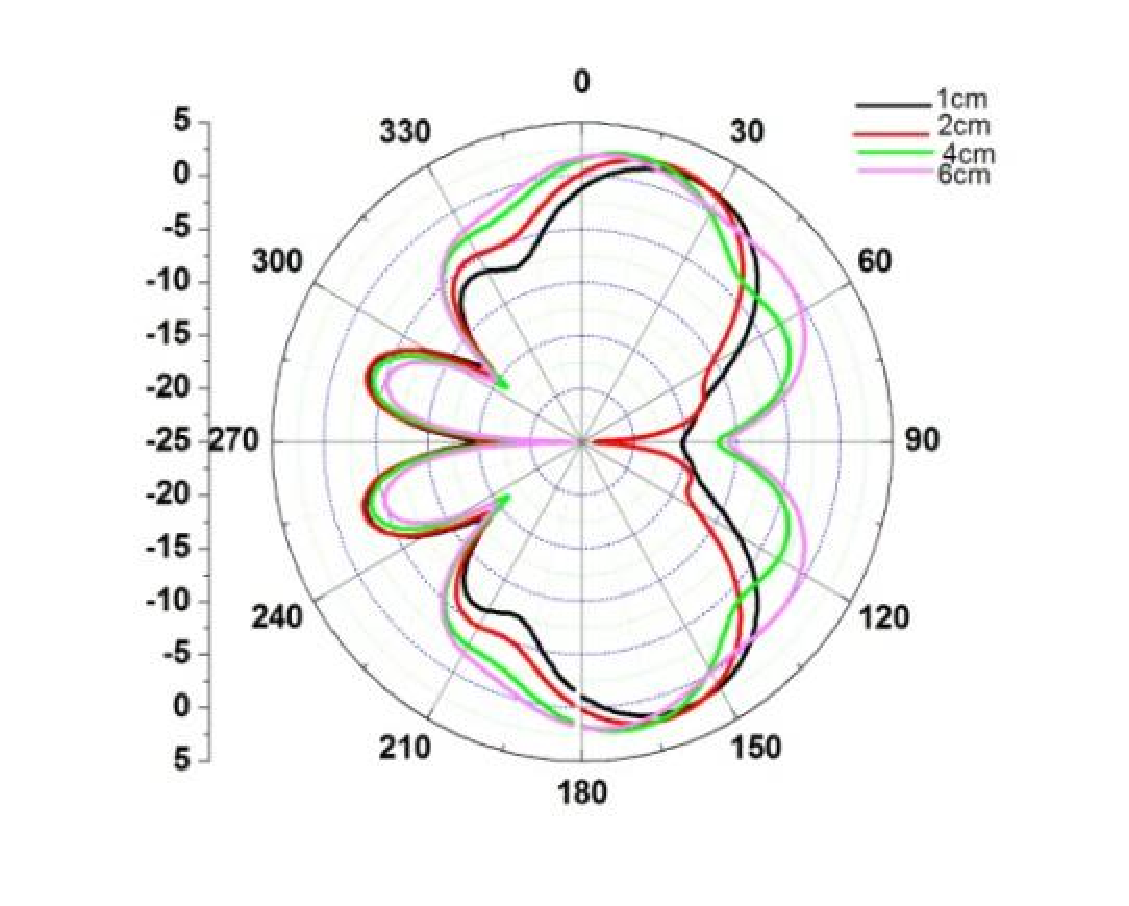
\includegraphics[width=\textwidth]{figs/10b.eps}
\caption{Vertical polarization of E-plane }
\label{fig:b}
\end{subfigure}
\begin{subfigure}[b]{0.24\textwidth}
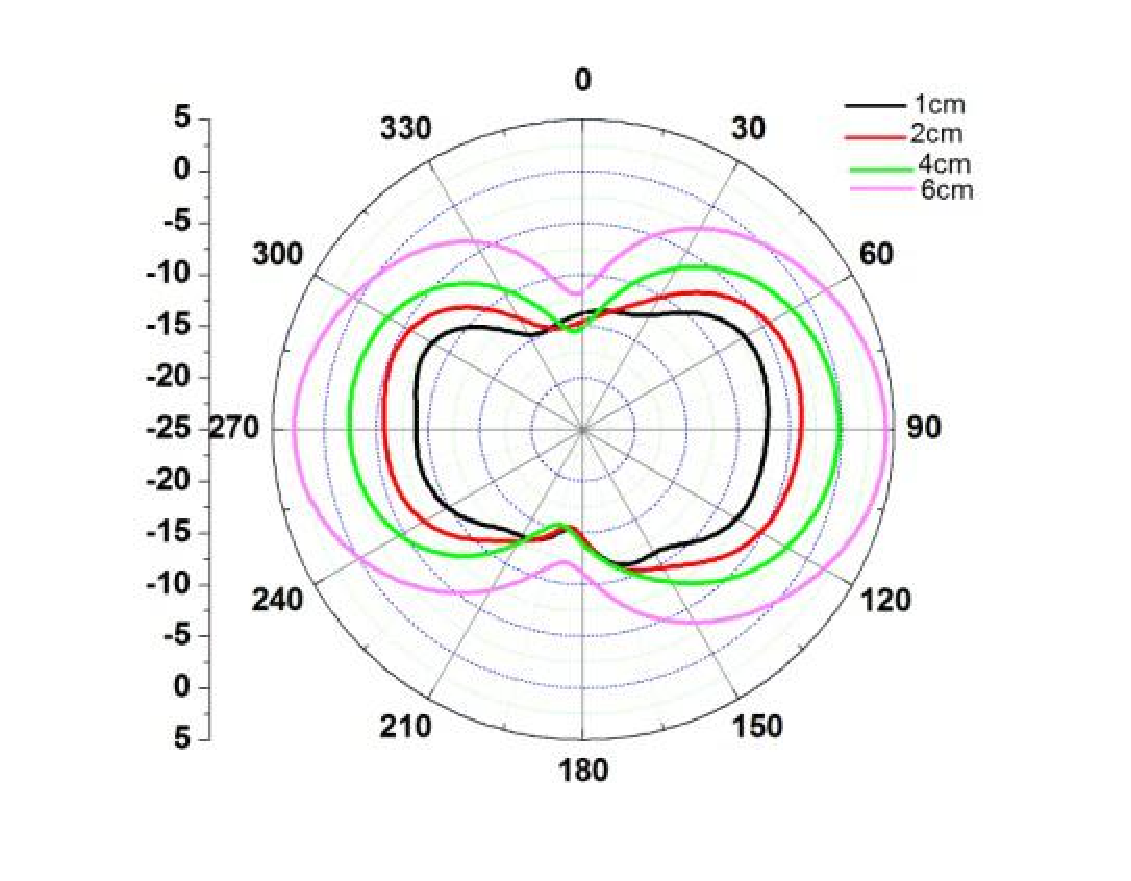
\includegraphics[width=\textwidth]{figs/10d.eps}
\caption{Horizontal polarization of H-plane}
\label{fig:d}	
\end{subfigure}
\begin{subfigure}[b]{0.24\textwidth}
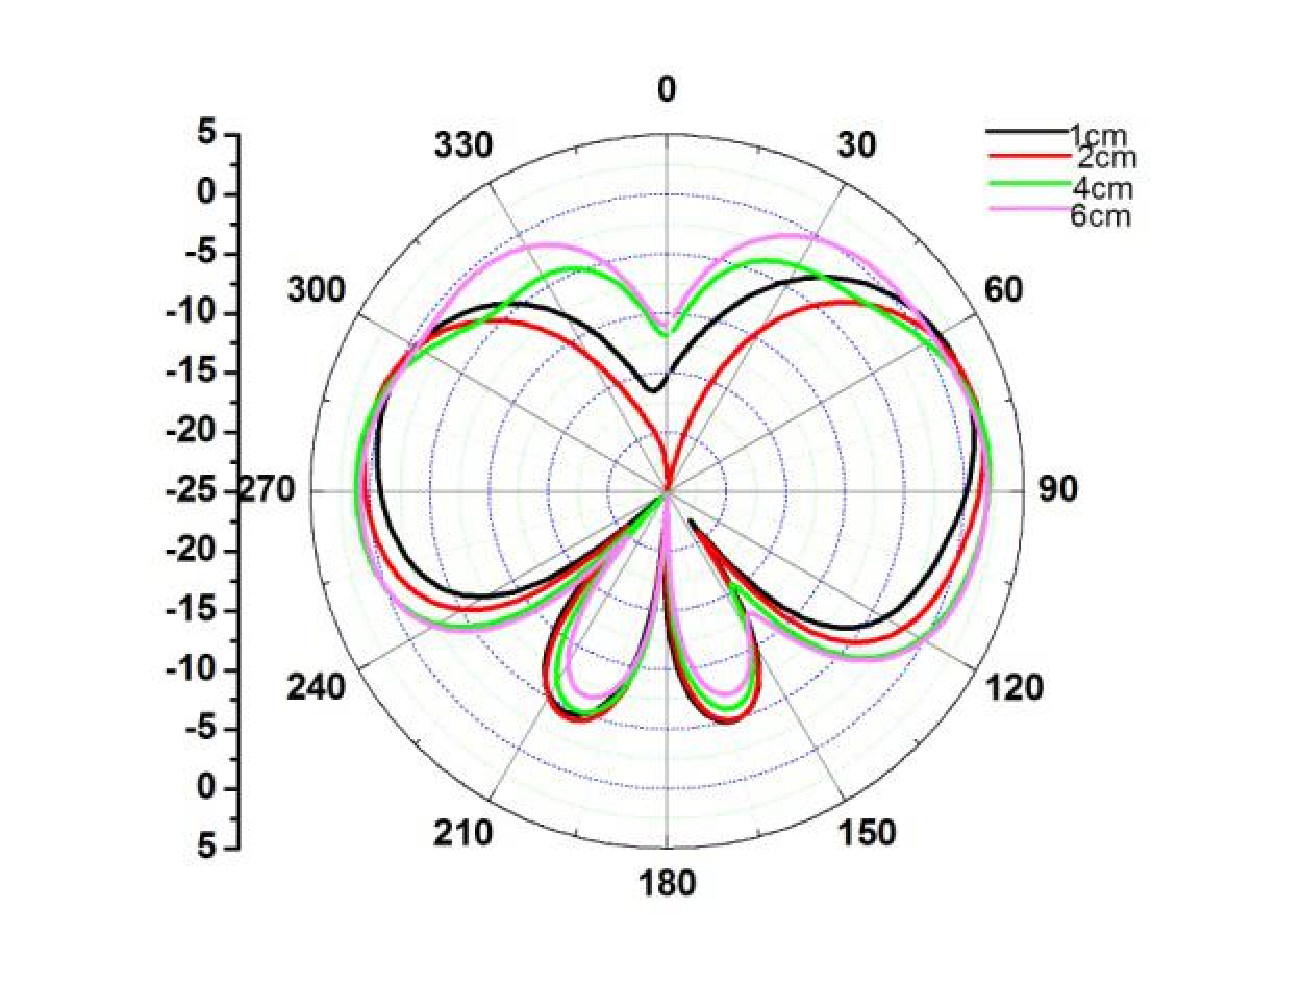
\includegraphics[width=\textwidth]{figs/10e.eps}
\caption{Vertical polarization of H-plane}
\label{fig:e}	
\end{subfigure}
\begin{subfigure}[b]{0.24\textwidth}
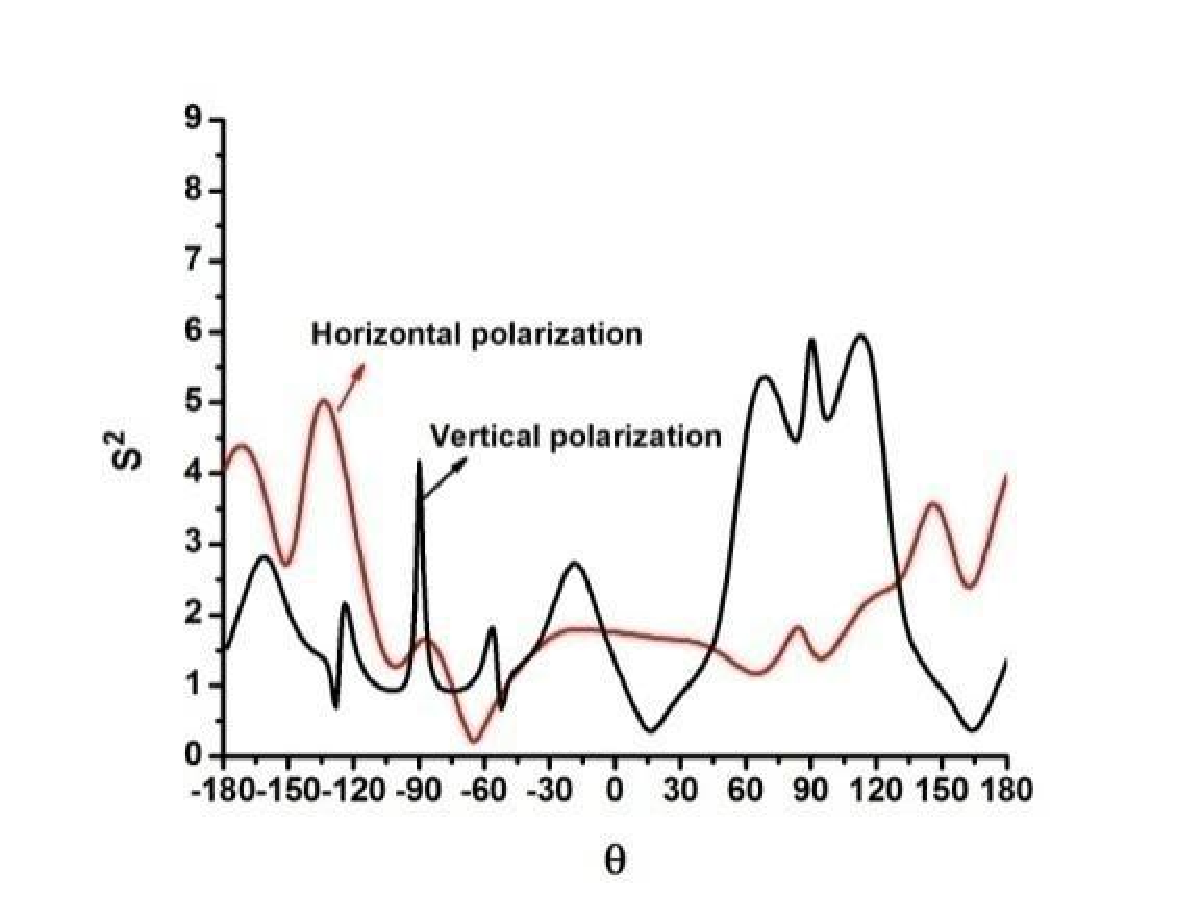
\includegraphics[width=\textwidth]{figs/10c.eps}
\caption{E-plane}
\label{fig:c}	
\end{subfigure}
\begin{subfigure}[b]{0.24\textwidth}
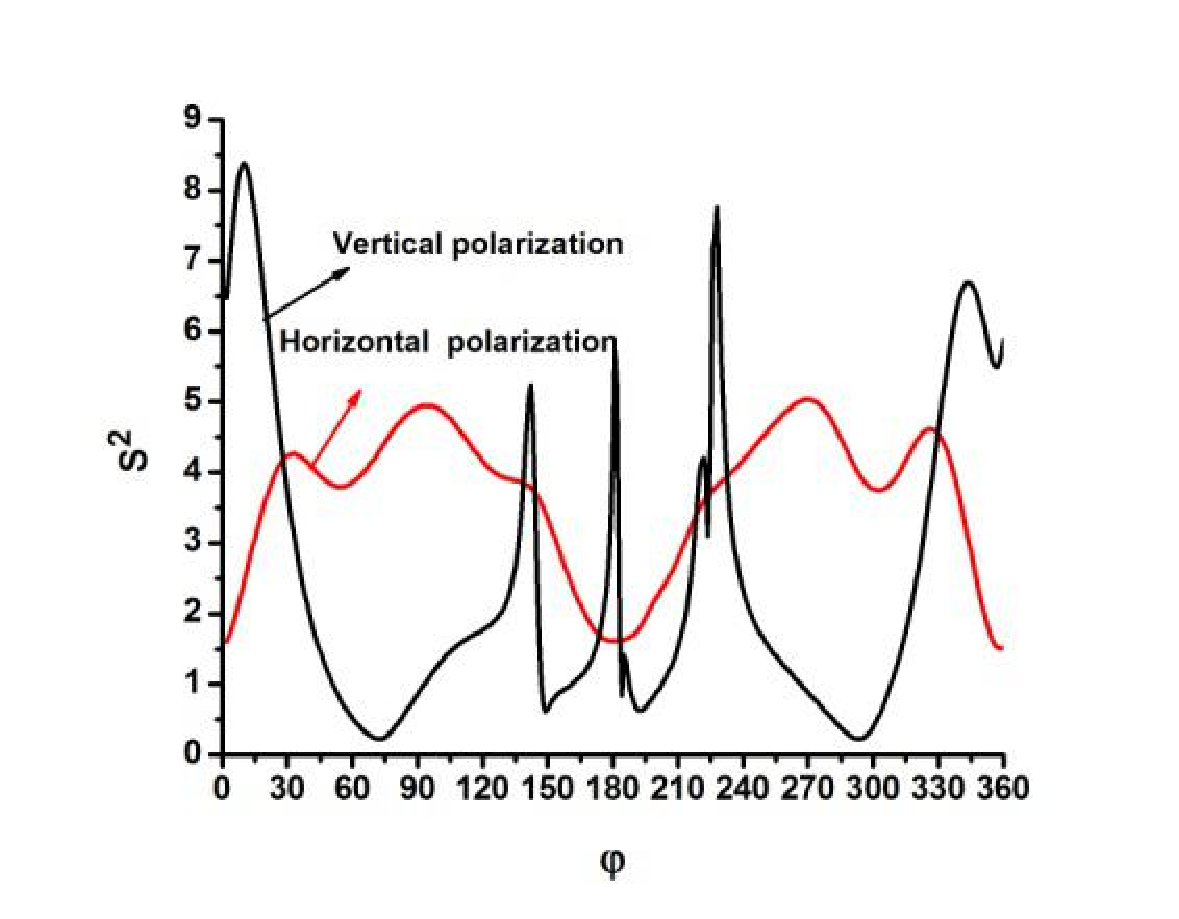
\includegraphics[width=\textwidth]{figs/10f.eps}
\caption{H-plane}
\label{fig:f}	
\end{subfigure}
\caption{Directional gain changes at different distances}
\label{fig:10}
\end{figure}
When \textit{d}=5.5cm, S11 takes the minimum. When 1cm$<\textit{d}<$2.5cm, S11 of vertically polarized is always smaller than horizontal polarization, and the bandwidth is always wider than horizontal polarization. In this range, the antenna is more suitable for placing on the surface of the human body in vertically polarized. When \textit{d}=0.5cm, S11 of vertical polarization take the maximum and the bandwidth is the narrowest, so the antenna is not suitable for placing on human body surface. The S11 curve of horizontal polarization is flat and when \textit{d}=4cm, \textit{B} reaches the maximum, so the antenna is most suitable to place on human body surface.

For the horizontal polarization, the square gain distributions at different distances are relatively uniform and not sensitive to distance. For E-plane pattern of vertical polarization, when $30\,^{\circ}$\textless$\varphi$\textless$150\,^{\circ}$, $S^{2}$\textgreater4, The gain difference at different distances is relatively large, the antenna direction gain is more sensitive to the distance factor than the other position. For H-plane pattern, when $130\,^{\circ}$\textless$\varphi$\textless$180\,^{\circ}$, $0\,^{\circ}$\textless$\varphi$\textless$30\,^{\circ}$, $225\,^{\circ}$\textless$\varphi$\textless$240\,^{\circ}$, $330\,^{\circ}$\textless$\varphi$\textless$360\,^{\circ}$, $S^{2}$\textgreater4, the antenna direction gain is more sensitive to the distance factor.
\begin{figure}[!htb]
\centering
\begin{subfigure}[b]{0.24\textwidth}
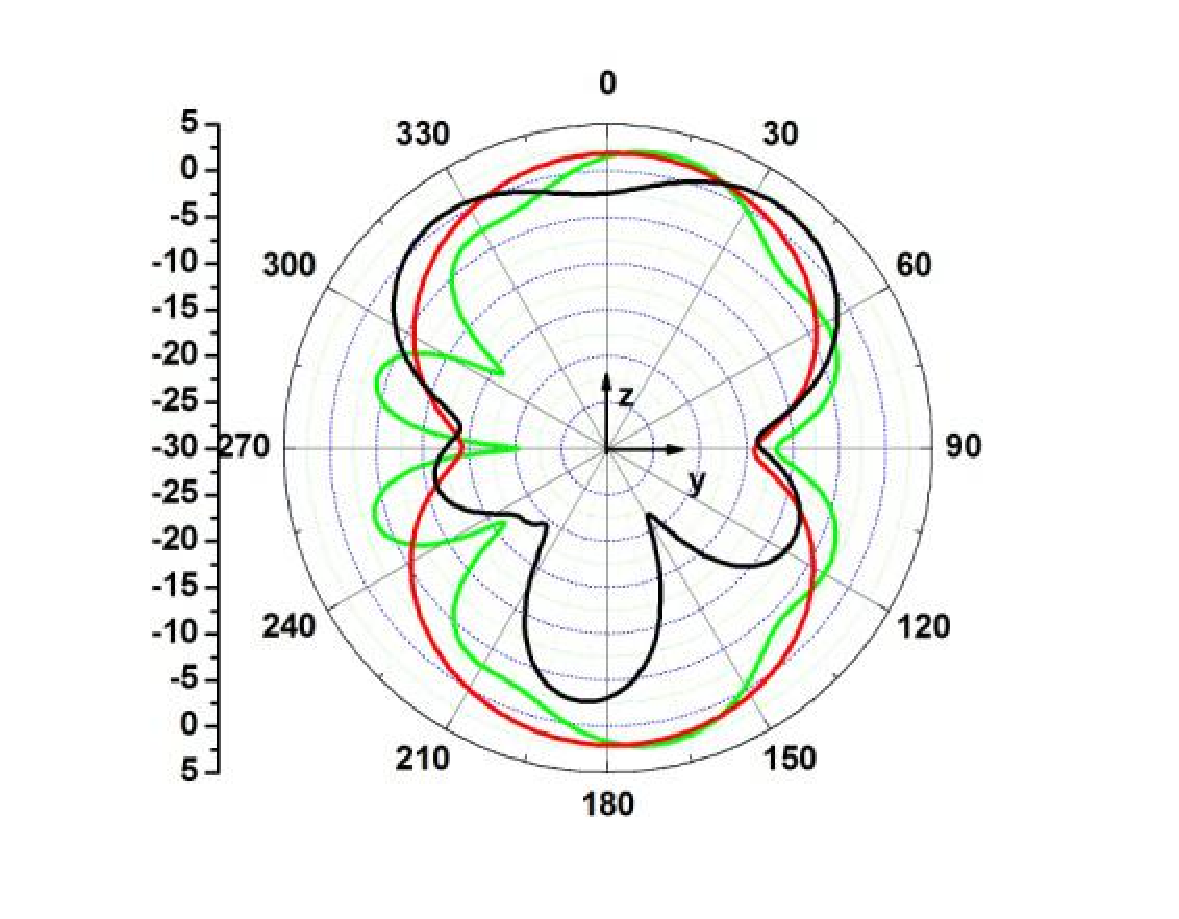
\includegraphics[width=\textwidth]{figs/11a.eps}
\caption{E-plane}
\label{fig:a}	
\end{subfigure}		
\begin{subfigure}[b]{0.24\textwidth}
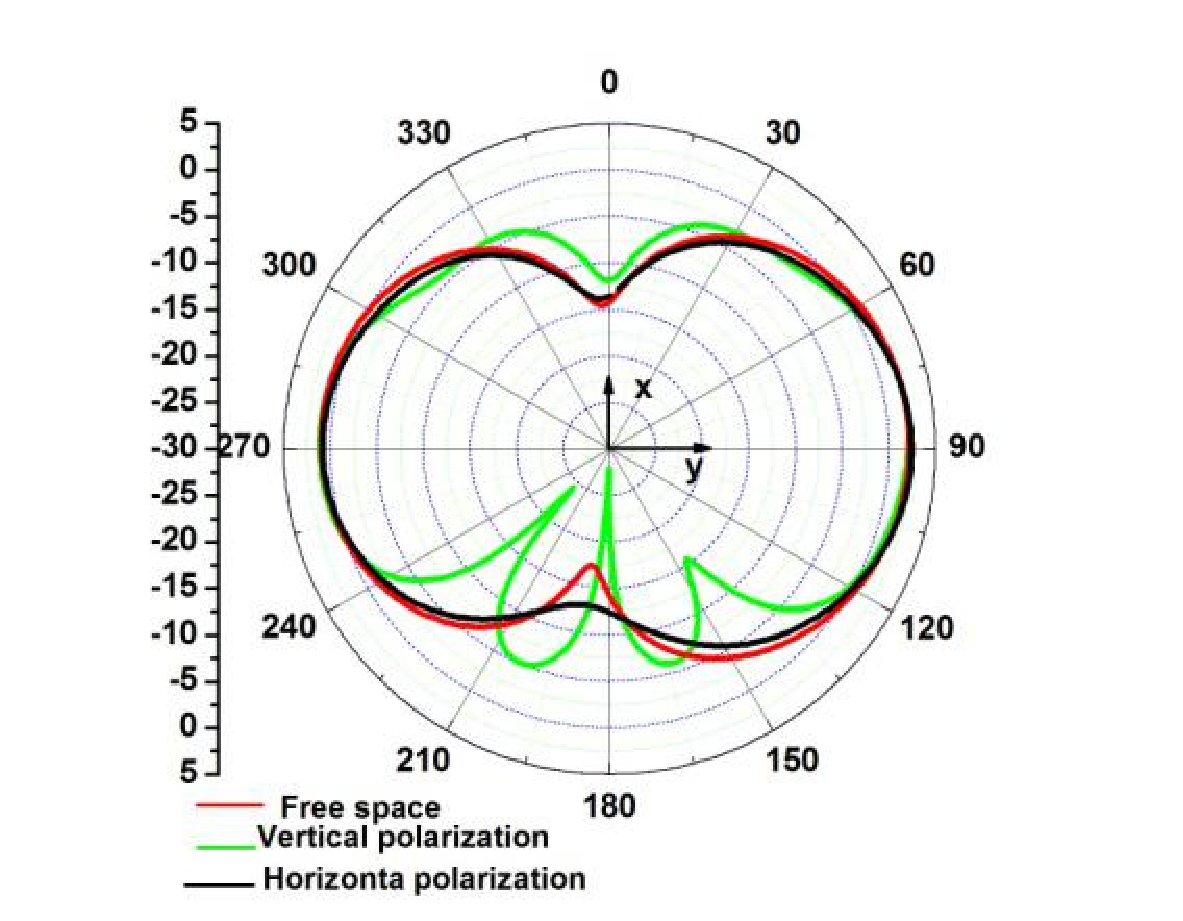
\includegraphics[width=\textwidth]{figs/11c.eps}
\caption{H-plane}
\label{fig:c}	
\end{subfigure}
\begin{subfigure}[b]{0.24\textwidth}
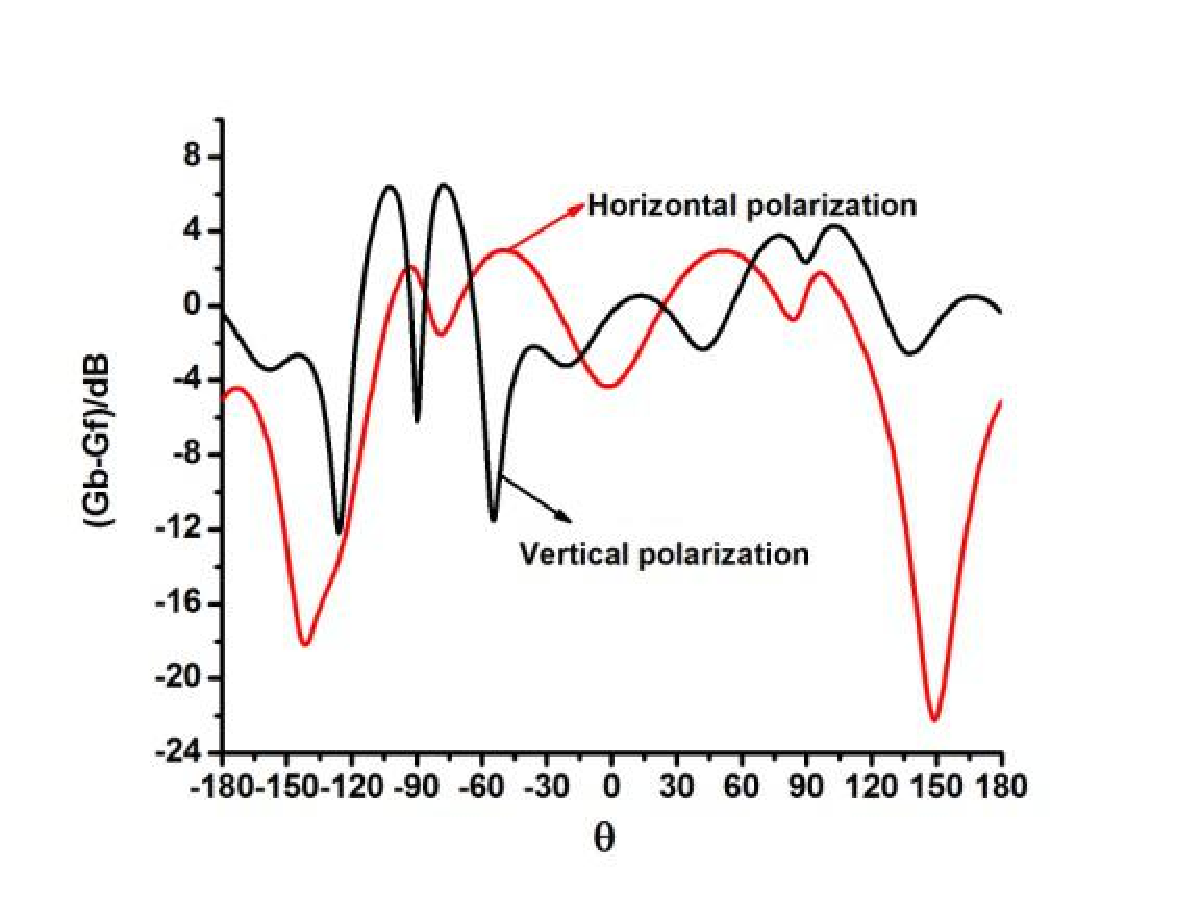
\includegraphics[width=\textwidth]{figs/11b.eps}
\caption{Differential gain of E-plane }
\label{fig:b}
\end{subfigure}
\begin{subfigure}[b]{0.24\textwidth}
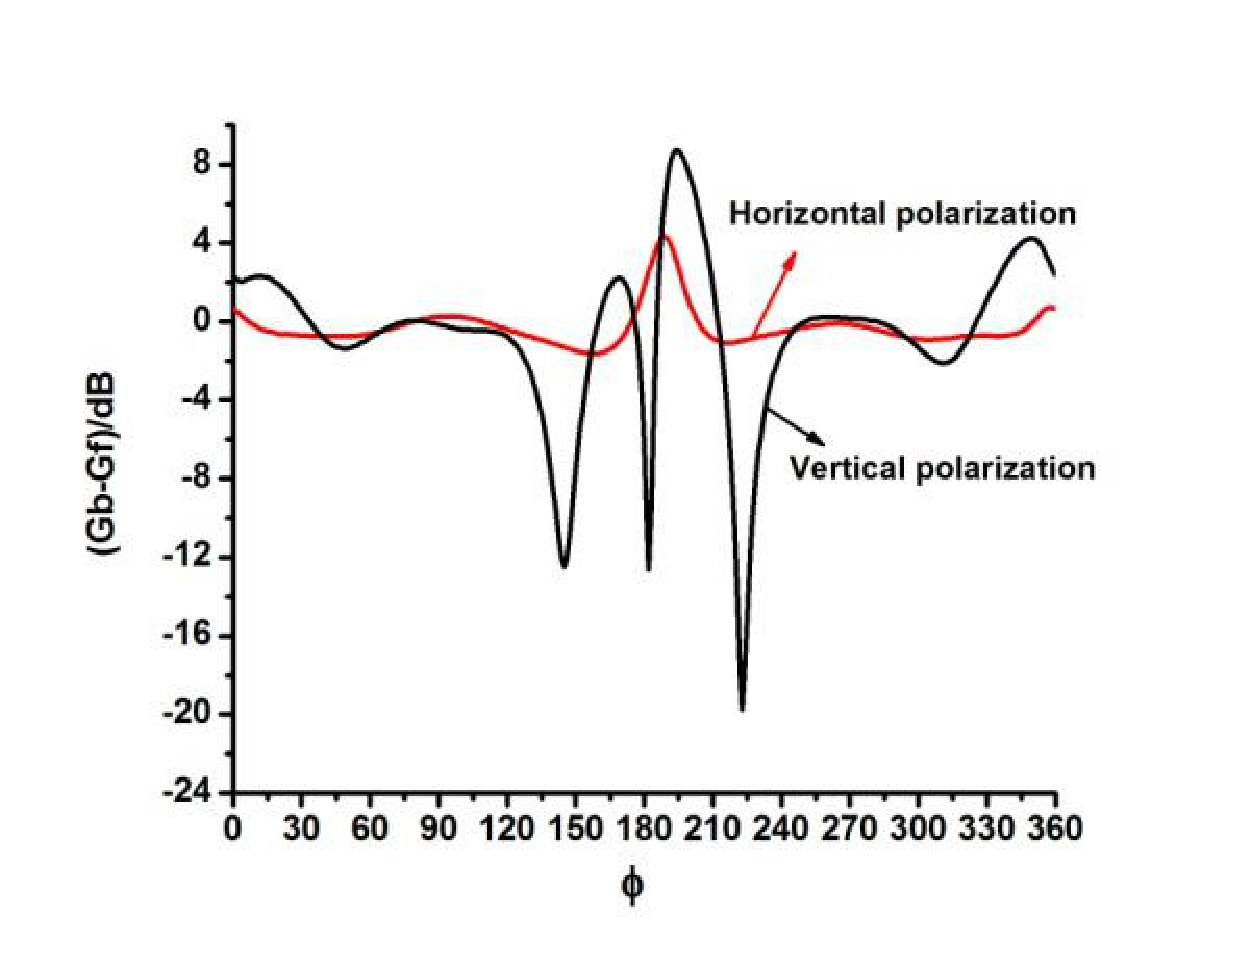
\includegraphics[width=\textwidth]{figs/11d.eps}
\caption{Differential gain of H-plane}
\label{fig:d}	
\end{subfigure}
\caption{Antenna gain pattern}
\label{fig:11}
\end{figure}
fig. \ref{fig:10} shows the radiation pattern of the antenna in free space and after loading body model. Horizontal polarization and vertical polarization were selected 5.5cm and 4cm respectively as the research focus.

The gain pattern of horizontal polarization and vertical polarization after loading human body model is symmetrically distributed with  $0\,^{\circ}$ and $90\,^{\circ}$ respectively. For horizontal polarization, the fitted curve equation of gain difference is
\begin{equation}
\label{eq:eps_5}
y[dB]=-4.5676x^2-0.0018x+1.1592, x[cm]
\end{equation}
At the position of $-180\,^{\circ}$\textless$\theta$\textless$-110\,^{\circ}$, $110\,^{\circ}$\textless$\theta$\textless$180\,^{\circ}$, $\mid$$G_{b}$-$G_{f}$$\mid$\textgreater4, the human body has a significant effect on antenna gain pattern. When $\theta$=$150\,^{\circ}$, $\mid$$G_{b}$-$G_{f}$$\mid$ takes the maximum, the human body has the greatest effect on antenna gain pattern. For vertical polarization, at the position of$-135\,^{\circ}$\textless$\theta$\textless$120\,^{\circ}$, $-65\,^{\circ}$\textless$\theta$\textless$-45\,^{\circ}$, $\mid$$G_{b}$-$G_{f}$$\mid$\textgreater6, the effect of the body on antenna gain pattern is obvious; when $\theta$=$130\,^{\circ}$and $\theta$=$550\,^{\circ}$, $\mid$$G_{b}$-$G_{f}$$\mid$=12, reaches the maximum, human body has the greatest effect on antenna gain pattern.

For H-plane gain pattern of the horizontal polarization, the gain curve is always gentle and the body has little effect on antenna gain pattern. For vertical polarization, the curve fluctuates obviously at the position of $145\,^{\circ}$\textless$\theta$\textless$230\,^{\circ}$, the human body has great effect on antenna. $\mid$$G_{b}$-$G_{f}$$\mid$ takes the maximum and the human body has the most obvious effect on antenna.

\subsubsection{Printed dipole}
\begin{figure}[!htb]
\centering
\begin{subfigure}[b]{0.4\textwidth}
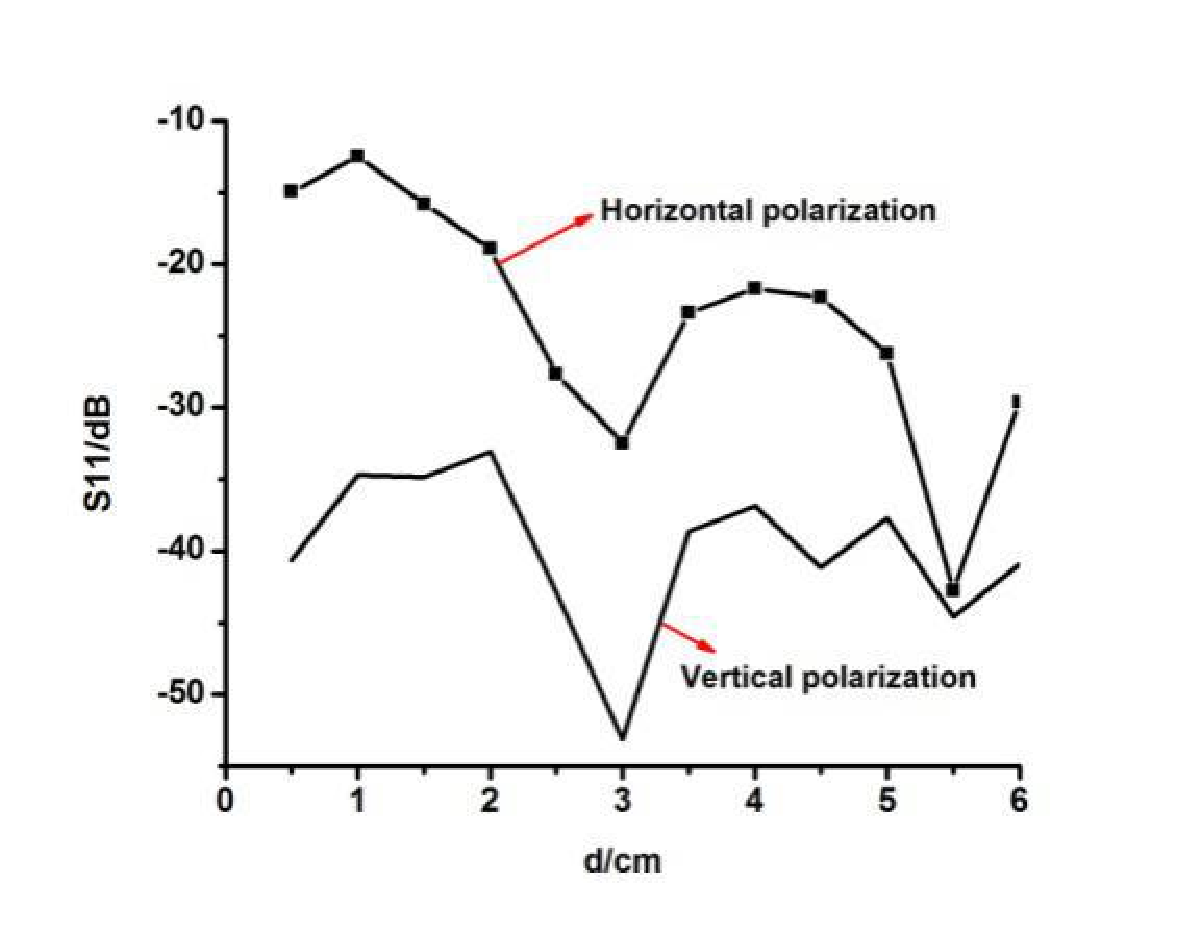
\includegraphics[width=\textwidth]{figs/12a.eps}
\caption{S11 changes}
\label{fig:a}	
\end{subfigure}		
\begin{subfigure}[b]{0.4\textwidth}
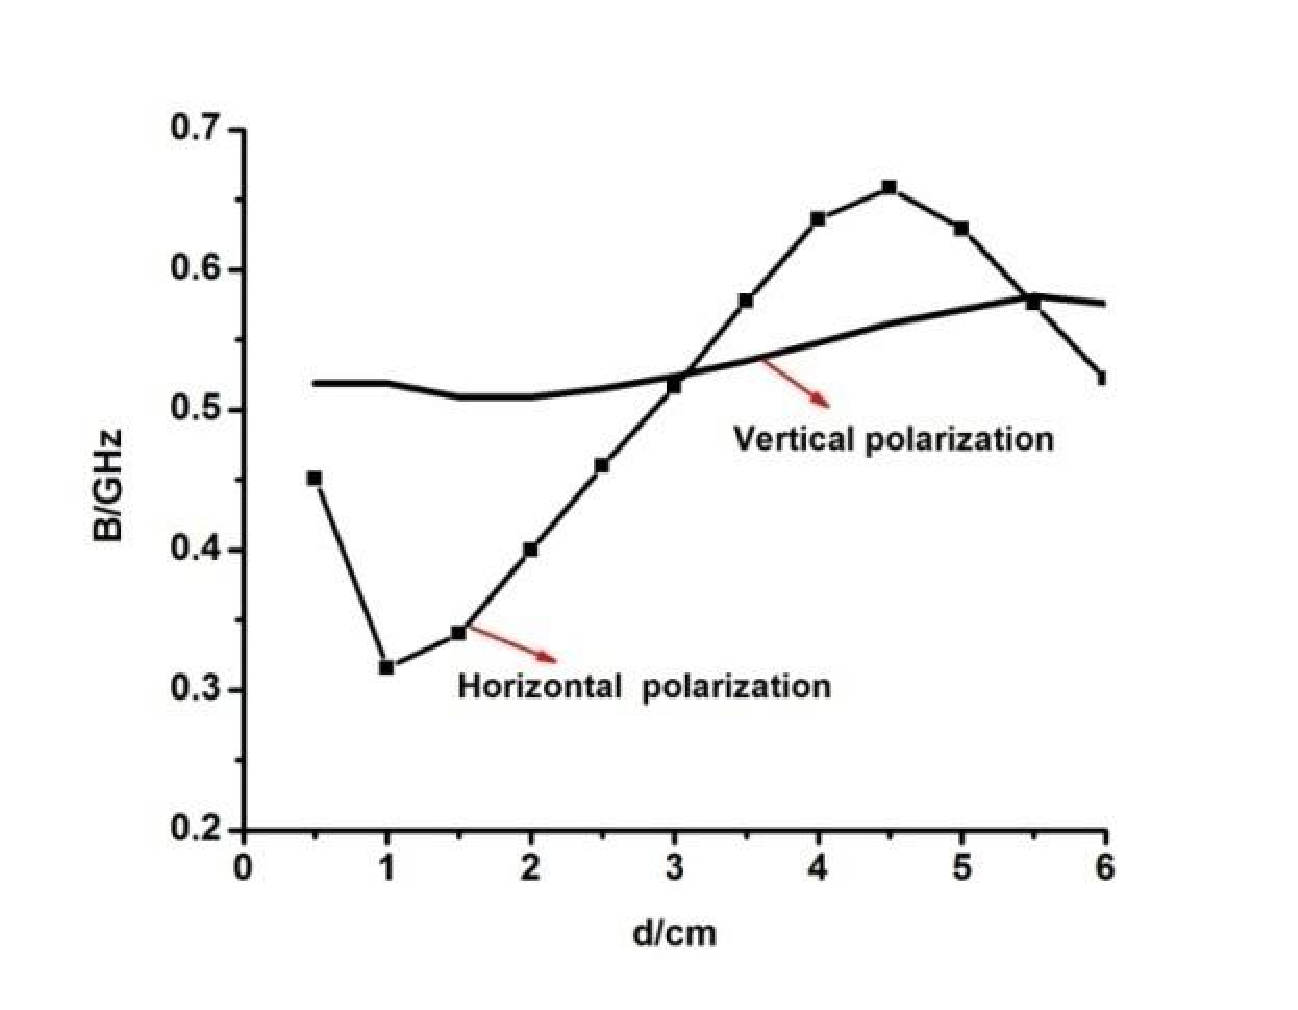
\includegraphics[width=\textwidth]{figs/12b.eps}
\caption{B changes}
\label{fig:b}
\end{subfigure}
\caption{Comparison of S11 and B of horizontal polarization and vertical polarization with different \textit{d}}
\label{fig:12}
\end{figure}
For horizontal polarization, the fitting curve equation of bandwidth is
\begin{equation}
\label{eq:eps_6}
y[dB]=0.014x+0.4937, x[cm]
\end{equation}
When \textit{d}=1cm, the bandwidth is narrowest, the antenna is not suitable for placing on body surface at this time. For vertical polarization, the fitted curve equation of bandwidth is
\begin{equation}
\label{eq:eps_7}
y[dB]=-0.0153x^2-0.2802x+0.52222, x[cm]
\end{equation}
At the range of all distances, when \textit{d}=3cm, S11 takes the minimum, so when the antenna placed 3cm near the body surface in vertical polarization, the antenna performance is the best. We can see form the S11 curve, the trend of vertical polarization and horizontal polarization is consistent, and the fitting curve equation is
\begin{equation}
\label{eq:eps_8}
y[dB]=-0.838x-37.197, x[cm]
\end{equation}
\begin{equation}
\label{eq:eps_9}
y[dB]=-3.4777X-12.723, x[cm]
\end{equation}
\begin{figure}[!htb]
\centering
\begin{subfigure}[b]{0.24\textwidth}
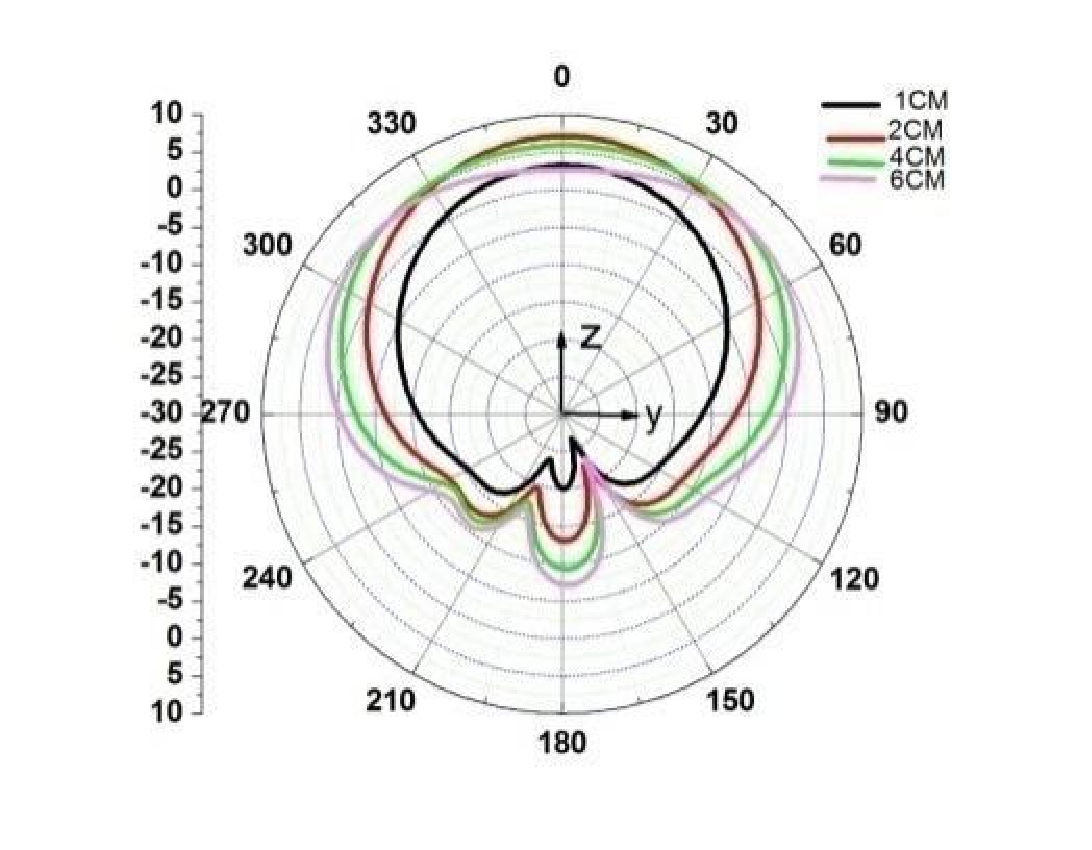
\includegraphics[width=\textwidth]{figs/13a.eps}
\caption{Horizontal polarization of E-plane}
\label{fig:13a}	
\end{subfigure}		
\begin{subfigure}[b]{0.24\textwidth}
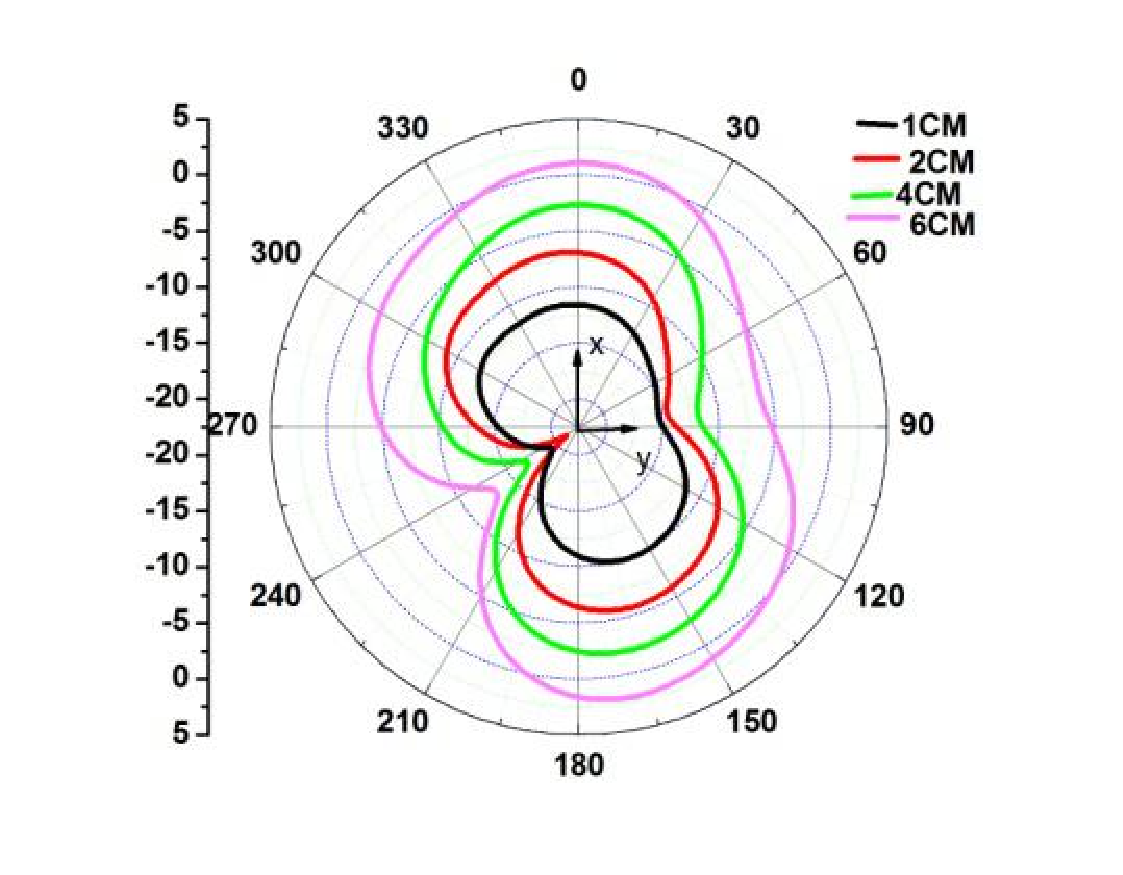
\includegraphics[width=\textwidth]{figs/13d.eps}
\caption{Horizontal polarization H-plane}
\label{fig:13d}	
\end{subfigure}
\begin{subfigure}[b]{0.24\textwidth}
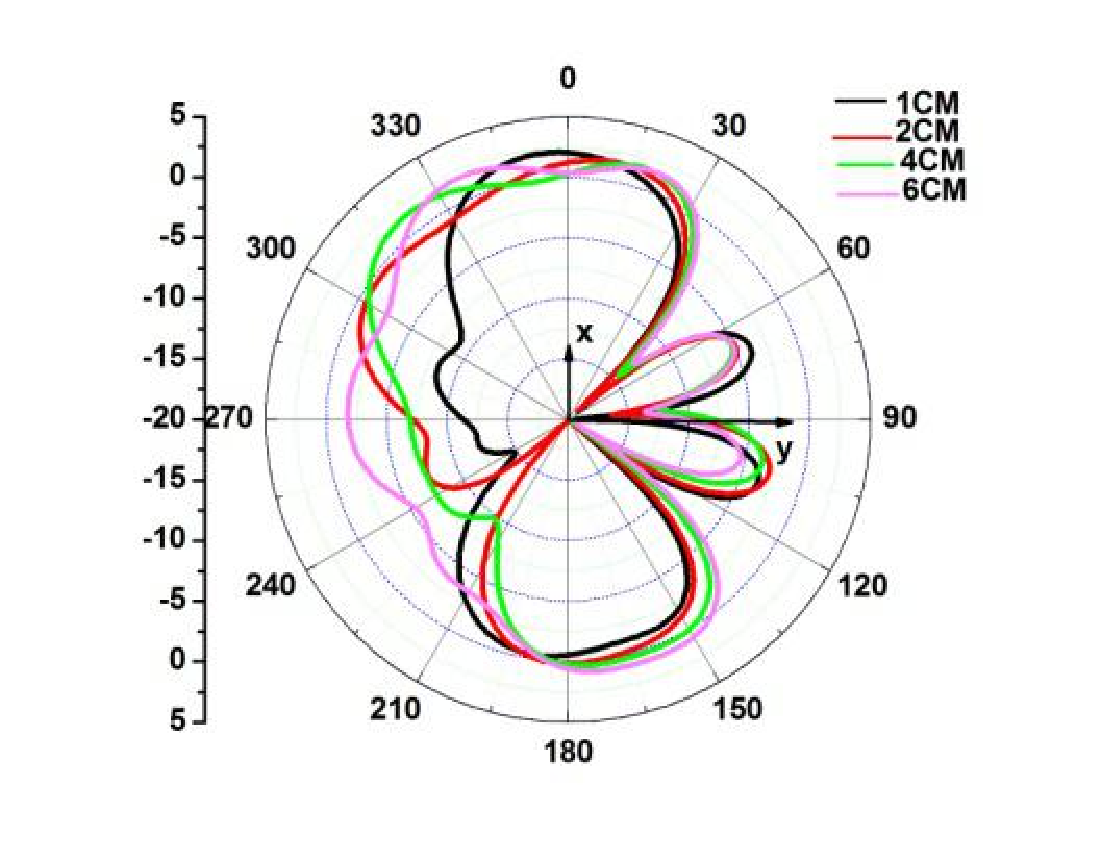
\includegraphics[width=\textwidth]{figs/13b.eps}
\caption{Vertical polarization E-plane}
\label{fig:13b}
\end{subfigure}
\begin{subfigure}[b]{0.24\textwidth}
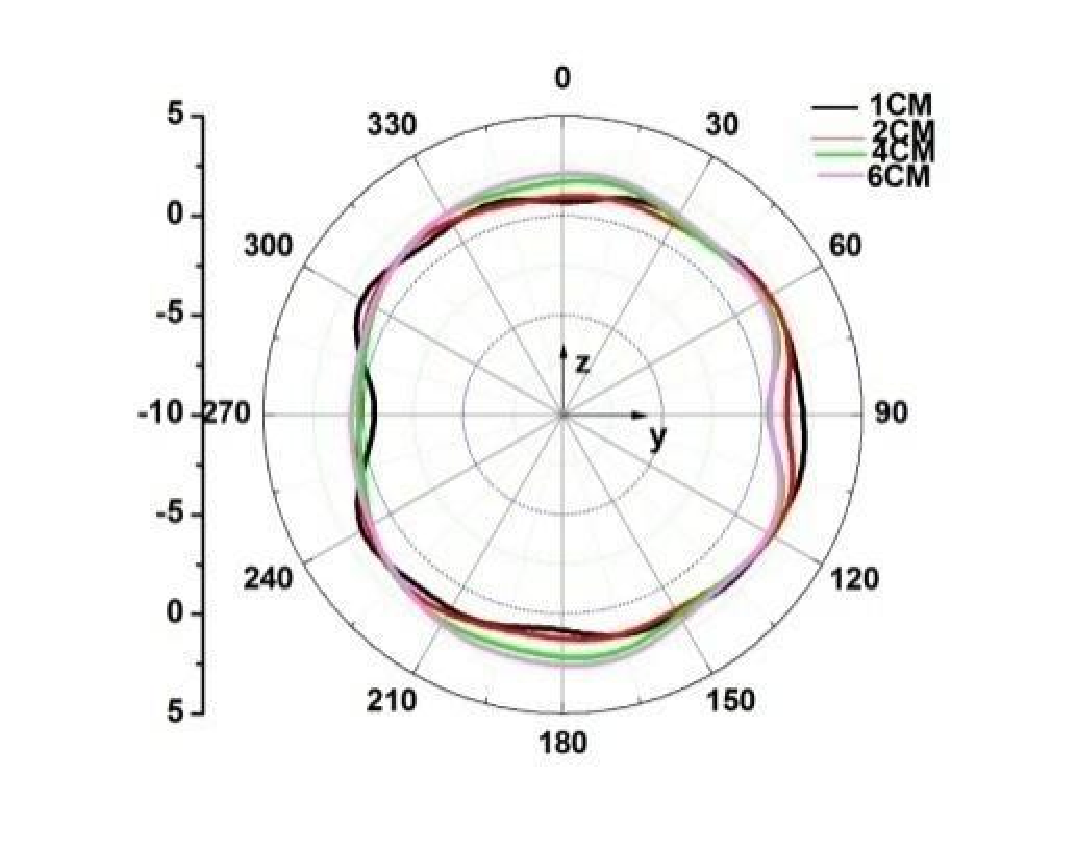
\includegraphics[width=\textwidth]{figs/13e.eps}
\caption{Vertical polarization of H-plane}
\label{fig:13e}	
\end{subfigure}
\begin{subfigure}[b]{0.24\textwidth}
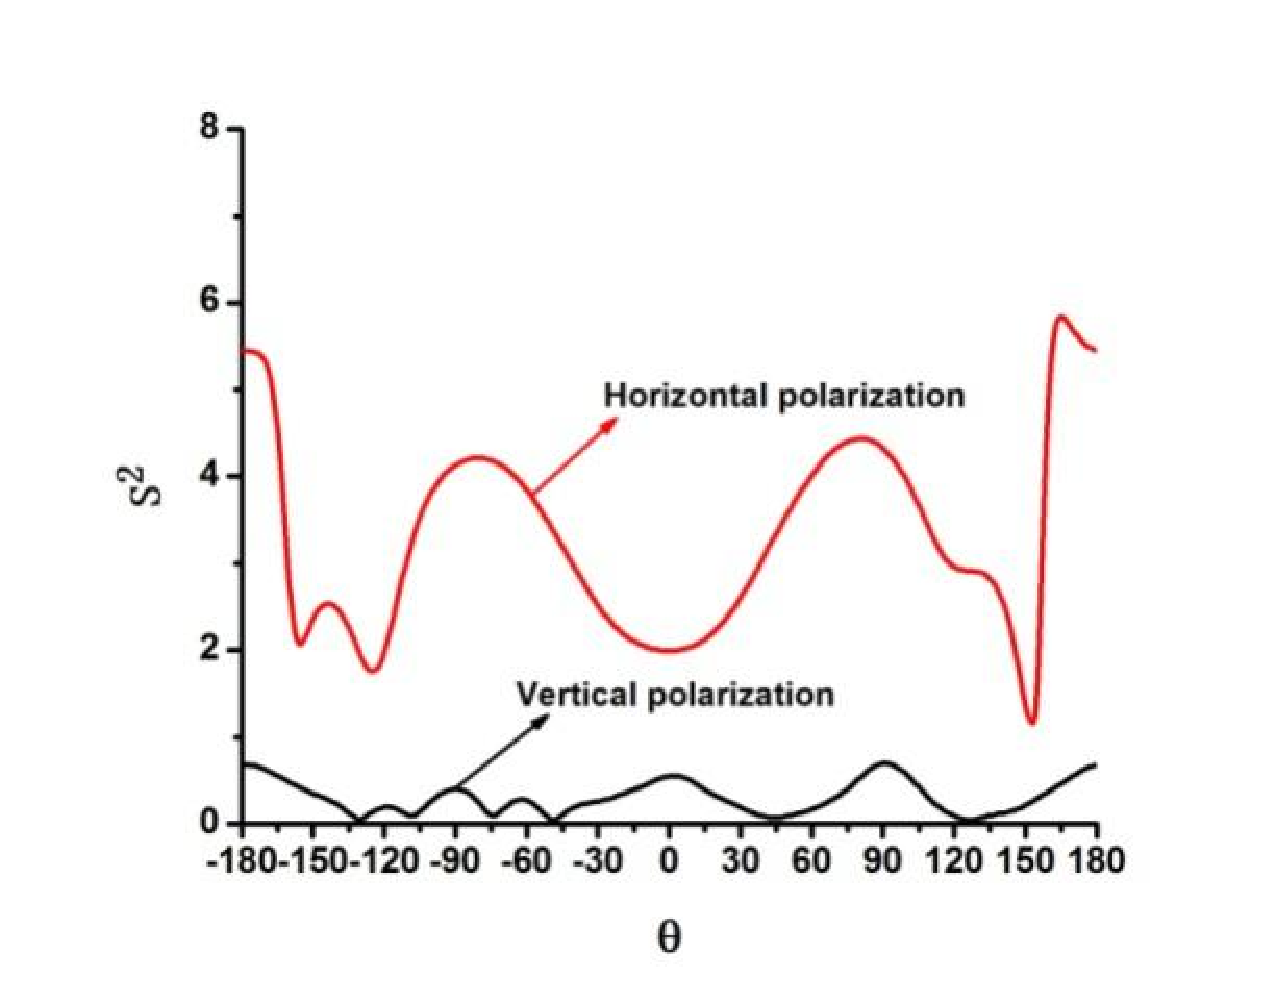
\includegraphics[width=\textwidth]{figs/13c.eps}
\caption{E-plane}
\label{fig:13c}	
\end{subfigure}
\begin{subfigure}[b]{0.24\textwidth}
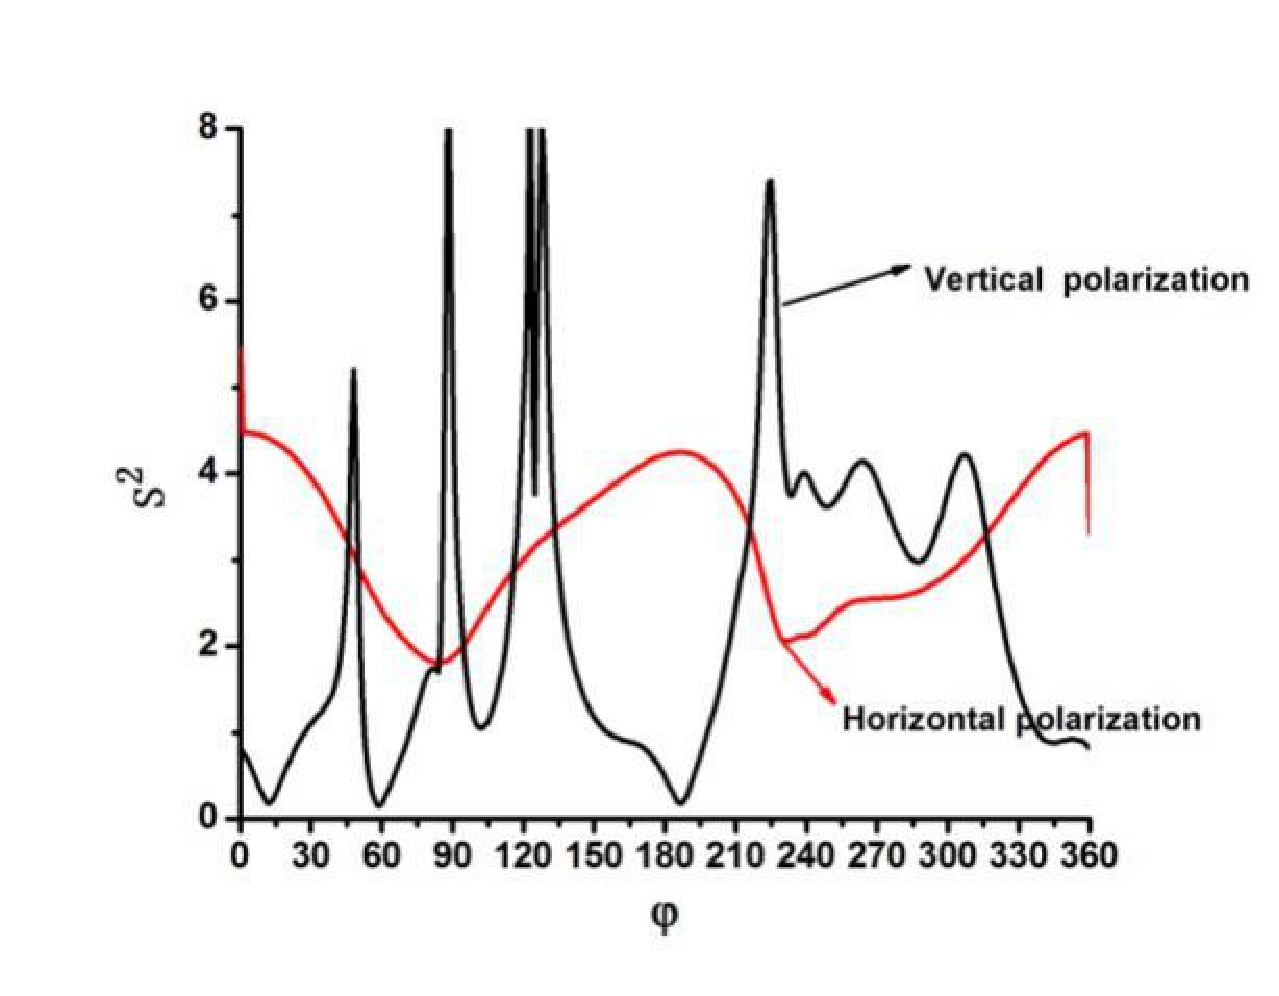
\includegraphics[width=\textwidth]{figs/13f.eps}
\caption{H-plane}
\label{fig:13f}	
\end{subfigure}
\caption{Comparison of gain pattern of horizontal polarization and vertical polarization of \textit{d}}
\label{fig:13}
\end{figure}
Horizontal polarization and vertical polarization take the minimum and maximum at \textit{d}=3cm and \textit{d}=5.5cm respectively. S11 of horizontal polarization is always greater than vertical polarization. When 0cm$<\textit{d}<$3cm, the bandwidth of vertical polarization is always greater than horizontal Polarization. Therefore, in this range of \textit{d}, the antenna is more suitable for vertical polarization.
For horizontal polarization, as shown in fig. \ref{fig:13a} and fig. \ref{fig:13d}, the directional gain distributions at different distances are relatively uniform and are not sensitive to d; but within the range of \textit{$\theta$} and \textit{$\varphi$}, 2\textless$S^{2}$\textless7, $S^{2}$ is large and the difference in gain is relatively large at different distances in the same direction.

For vertical polarization, as shown in fig. \ref{fig:13b} and fig. \ref{fig:13e}, the E-plane pattern is stable and is not sensitive to \textit{d}. At the position of $85\,^{\circ}$\textless$\varphi$\textless$90\,^{\circ}$, $120\,^{\circ}$\textless$\varphi$\textless$130\,^{\circ}$, $220\,^{\circ}$\textless$\varphi$\textless$230\,^{\circ}$, $S^{2}$\textgreater7, the difference of H-plane pattern of \textit{d} is relatively great, the antenna direction gain is more sensitive to \textit{d}.
\begin{figure}[!htb]
\centering
\begin{subfigure}[b]{0.24\textwidth}
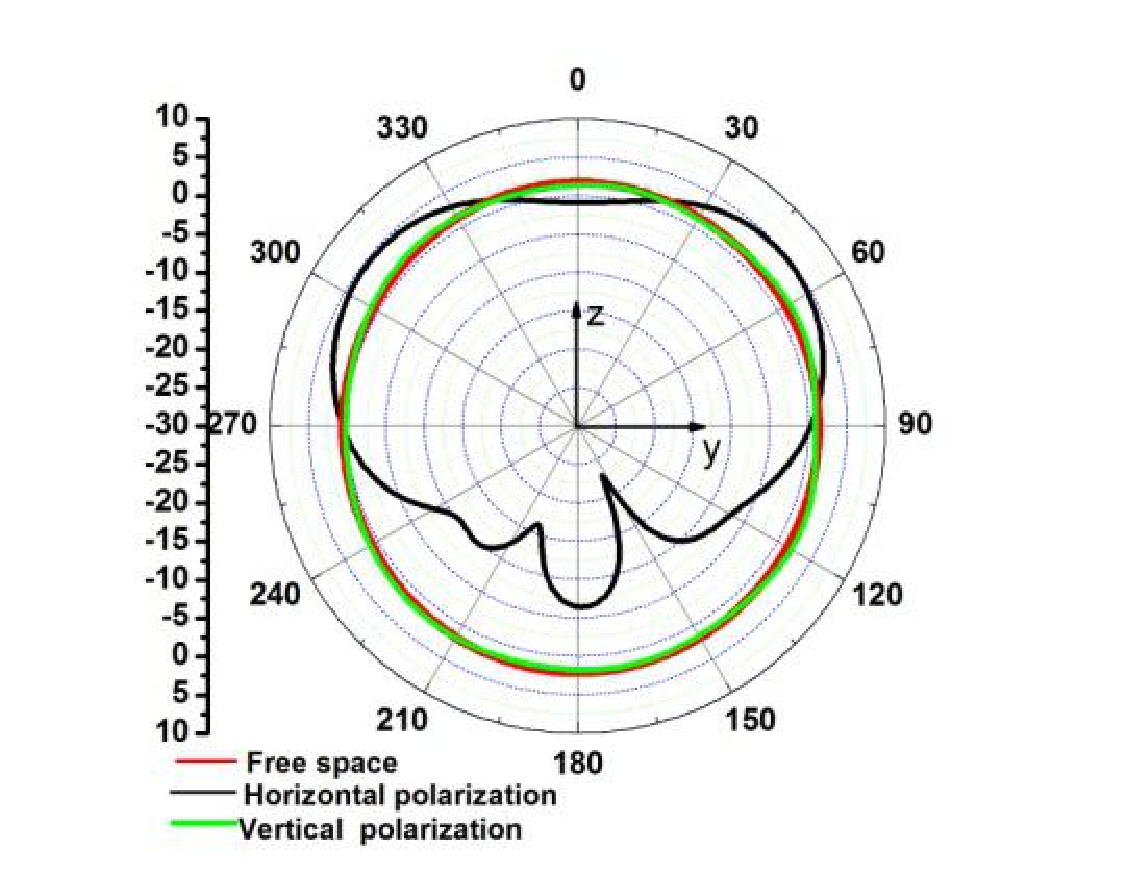
\includegraphics[width=\textwidth]{figs/14a.eps}
\caption{E-plane}
\label{fig:a}	
\end{subfigure}		
\begin{subfigure}[b]{0.24\textwidth}
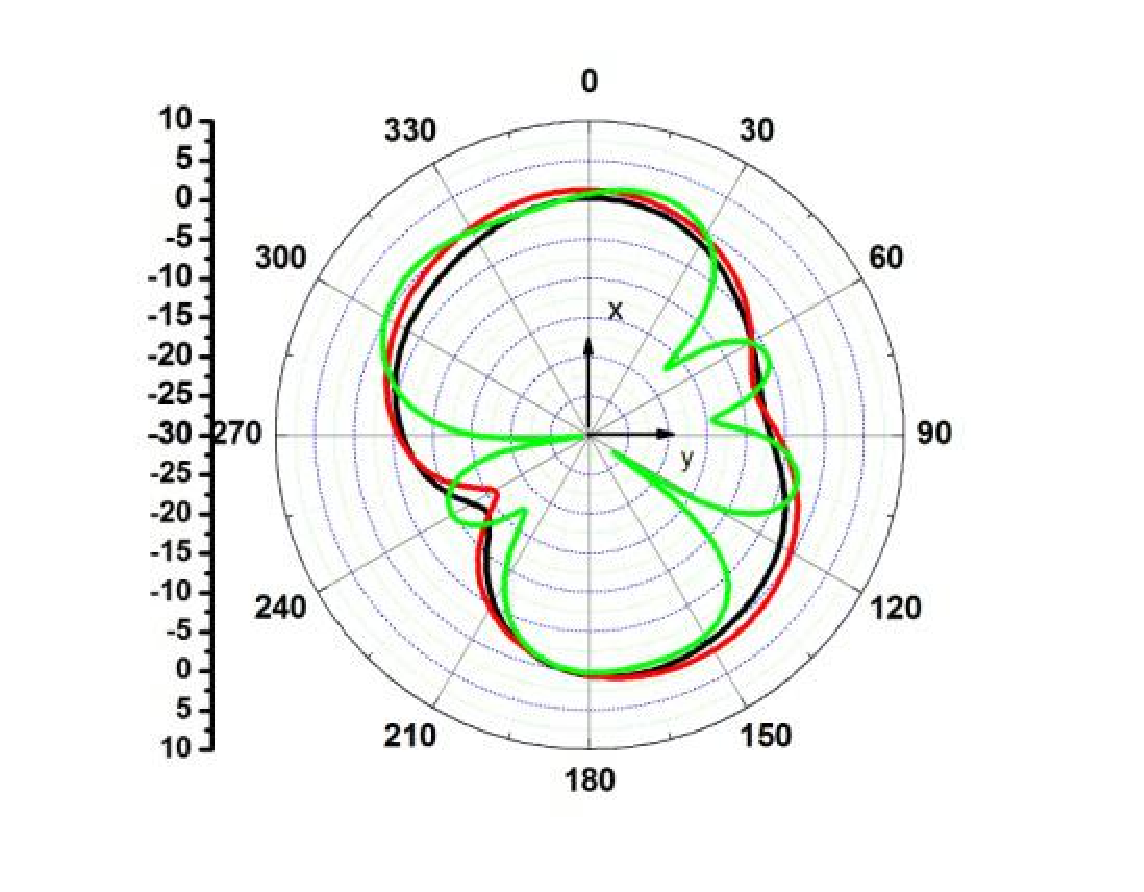
\includegraphics[width=\textwidth]{figs/14c.eps}
\caption{H-plane}
\label{fig:c}	
\end{subfigure}
\begin{subfigure}[b]{0.24\textwidth}
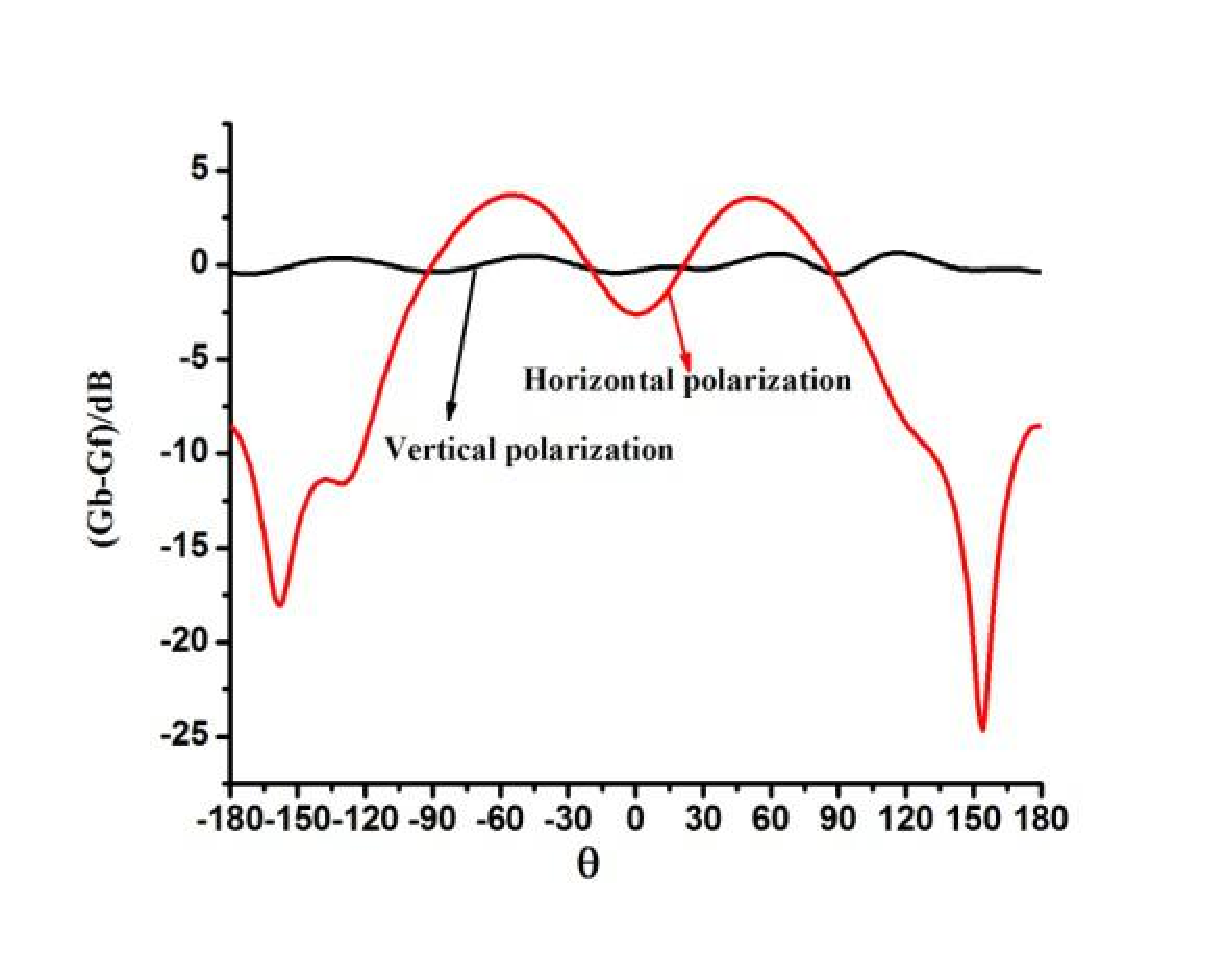
\includegraphics[width=\textwidth]{figs/14b.eps}
\caption{Differential gain of E-plane }
\label{fig:b}
\end{subfigure}
\begin{subfigure}[b]{0.24\textwidth}
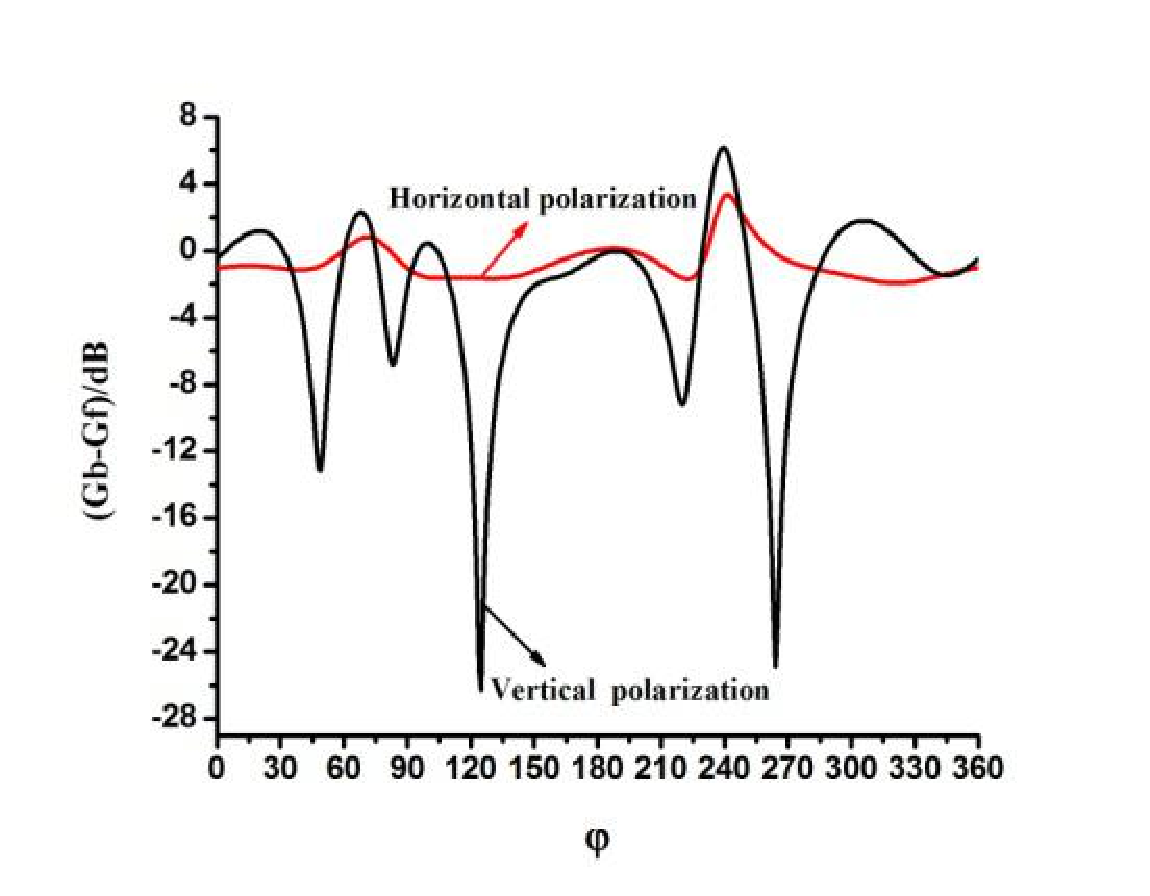
\includegraphics[width=\textwidth]{figs/14d.eps}
\caption{Differential gain of H-plane}
\label{fig:d}	
\end{subfigure}
\caption{Antenna gain pattern}
\label{fig:14}
\end{figure}

Horizontal polarization and vertical polarization were selected 5.5cm and 3cm as the research respctively. The antenna performance of other \textit{d} is better and antenna radiation orientation is more obvious, the maximum gain reached 5dB.

For E-plane, the antenna polarization pattern of horizontal polarization and vertical polarization after loading human body is symmetrically distributed with $\theta$=$0\,^{\circ}$ and $\theta$=$90\,^{\circ}$ respectively. The E-plane pattern of vertical polarization after loading the human body is close to omnidirectional distribution of free space. For horizontal polarization, the fitted gain difference curve equation is
\begin{equation}
\label{eq:eps_10}
y[dB]=-0.0006078x^2-0.00243x+2.26111, x[cm]
\end{equation}
Due to the radiation of human body, at the position of $130\,^{\circ}$\textless$\theta$\textless$180\,^{\circ}$ and $-130\,^{\circ}$\textless$\theta$\textless$-180\,^{\circ}$ , the gain difference is relatively great and the human body has obvious effect on antenna gain pattern. The gain is enhanced at the position of $-90\,^{\circ}$\textless$\theta$\textless$-15\,^{\circ}$ and weakened at other position. For horizontal polarization, $\mid$$G_{b}$-$G_{f}$$\mid$\textless4dB, the human body has little effect on H-plane gain pattern; For vertical polarization, at the position of $40\,^{\circ}$\textless$\varphi$\textless$55\,^{\circ}$, $110\,^{\circ}$\textless$\varphi$\textless$135\,^{\circ}$, $210\,^{\circ}$\textless$\varphi$\textless$225\,^{\circ}$, $260\,^{\circ}$\textless$\varphi$\textless$270\,^{\circ}$, $\mid$$G_{b}$-$G_{f}$$\mid$\textgreater6dB, the human body has a great effect on antenna gain. When $\varphi$=$125\,^{\circ}$ and $\varphi$=$265\,^{\circ}$, $\mid$$G_{b}$-$G_{f}$$\mid$=26dB, taking the maximum and the gain is obviously reduced.

\section{Conclusion}
In this paper, three kinds of linearly polarized antennas operating at 2.45GHz are studied. The human body is loaded and simulated in the HFSS simulation software. After loading body model, when IFA placed on the surface of body in horizontal polarization, resonant frequency decreases at the range of 2.4GHz-2.5GHz with the increase of \textit{d}. For vertical polarization, the antenna resonant frequency is always moves around 2.45GHz and has no significant change. When MIFA placed on the surface of human body in horizontal polarization, the resonant frequency is shifted from 2.5GHz to 2.45GHz with the increases of \textit{d} and vertical polarization is contrary to horizontal polarization. When printed dipole placed on the surface of human body in horizontal polarization and vertical polarization, the antenna resonant frequency moved in the range of 2.3GHz-2.5GHz and 2.45GHz-2.5GHz, respectively. Due to the coupling effect of the human body, the antenna radiation pattern shows a certain orientation and the main lobe gain of the antenna is improved. The gain of the dipole and MIFA of vertical polarization is not sensitive to \textit{d}. The gain difference is great at different distances of the same direction for horizontal polarization and IFA is on the contrary and gain is not sensitive to \textit{d} when placed on body surface in horizontally polarization.

\ifCLASSOPTIONcaptionsoff
  \newpage
\fi




\begin{thebibliography}{1}
\bibitem{1}
Jensen M A, Rahmat-Samii Y. EM  interaction of handset antennas and a human in personal communications[J]. \emph{Proceedings of the IEEE},1995,83(1):1-17

\bibitem{2}
Iskander, M. E., Zhengqing Yun, and R.Quintero-Illera.``Polarization and human body effects on the microwave absorption in a human head exposed to radiation from handheld devices.''
\emph{IEEE Transactions on Microwave Theory and Techniques}, 2000, 48(11): 1979-1987.

\bibitem{3}
Hurme H, Salonen P, Rantanen J, et al. On the Study of Antenna Placement in a Smart Clothing[C]//\emph{Modelling and Simulation}, 2003: 1-6.

\bibitem{4}
Wei W Y, Gong D M, Chen B S. Antenna theory[M]. Xi��an: Publishing House of School of Electronic Engineering, Xidian University, 1994

\bibitem{5}
Klemm M, Troester G. Textile UWB antennas for wireless body area networks[J]. \emph{Transactions on Antennas and Propagation}, 2006, 54(11): 3192-3197.

\bibitem{6}
Wang Z, Zhang L, Psychoudakis D, et al. Flexible textile antennas for body-worn communication[C]//Antenna Technology (iWAT), \emph{2012 IEEE International Workshop on. IEEE}, 2012: 205-208.

\bibitem{7}
Wang Z, Zhang L, Bayram Y, et al.Embroidered conductive fibers on polymer composite for conformal antennas[J]. \emph{IEEE Transactions on Antennas and Propagation}, 2012, 60(9): 4141-4147.

\bibitem{8}
LI M Y, LIU M, Yang F.HFSS Antennas DESGIN[M]. Beijing: Publishing House of Electronic Industry, 2011:196-218, 51-53.

\bibitem{9}
Andersen A. Small size 2.4 GHz PCB antenna[J]. Texas Instruments, Application Note AN043, 2008.

\bibitem{10}
Psychoudakis D, Volakis J L. Conformal asymmetric meandered flare (AMF) antenna for body-worn applications[J].
\emph{IEEE Antennas and Wireless Propagation Letters}, 2009, 8: 931-934.

\bibitem{11}
Dimbylow P J, Gandhi O P. Finite-difference time-domain calculations of SAR in a realistic heterogeneous model of the head for plane-wave exposure from 600 MHz to 3 GHz[J]. \emph{Physics in Medicine and Biology}, 1991, 36(8): 1075.

\end{thebibliography}

% biography section
%
% If you have an EPS/PDF photo (graphicx package needed) extra braces are
% needed around the contents of the optional argument to biography to prevent
% the LaTeX parser from getting confused when it sees the complicated
% \includegraphics command within an optional argument. (You could create
% your own custom macro containing the \includegraphics command to make things
% simpler here.)
%\begin{IEEEbiography}[{\includegraphics[width=1in,height=1.25in,clip,keepaspectratio]{mshell}}]{Michael Shell}
% or if you just want to reserve a space for a photo:



% if you will not have a photo at all:

% insert where needed to balance the two columns on the last page with
% biographies
%\newpage



% You can push biographies down or up by placing
% a \vfill before or after them. The appropriate
% use of \vfill depends on what kind of text is
% on the last page and whether or not the columns
% are being equalized.

%\vfill

% Can be used to pull up biographies so that the bottom of the last one
% is flush with the other column.
%\enlargethispage{-5in}



% that's all folks
\end{document}


